\section{AirflowNetwork Model}\label{airflownetwork-model}

\subsection{Overview}\label{afn-overview}

The AirflowNetwork model provides the ability to simulate the performance of an air distribution system, including supply and return leaks, and calculate multizone airflows driven by outdoor wind and forced air during HVAC system operation. The pressure and airflow model described here was developed based on AIRNET (Walton 1989). This detailed model is used to simulate thermal conduction and air leakage losses for constant volume air distribution systems (e.g., in residential or light commercial buildings). The multizone airflow calculations are performed at the HVAC system time step which, among other benefits, allows for modeling hybrid ventilation systems.

\subsection{Model Description}\label{afn-model-description}

The input object AirflowNetwork:SimulationControl provides access to the airflow network method, which consists of a set of nodes connected by airflow components through linkages. The objects AirflowNetwork:Multizone:Zone, AirflowNetwork:Multizone:ExternalNode, and AirflowNetwork:Distribution:Node represent airflow nodes. The objects AirflowNetwork:Multizone:Surface and AirflowNetwork:Distribution:Linkage represent airflow linkages. The other objects with a relationship between pressure and airflow represent airflow components.

The AirflowNetwork model consists of three sequential steps:

\begin{itemize}
\item
  Pressure and airflow calculations
\item
  Node temperature and humidity calculations
\item
  Sensible and latent load calculations
\end{itemize}

The pressure and airflow calculations determine pressure at each node and airflow through each linkage given wind pressures and forced airflows. Based on the airflow calculated for each linkage, the model then calculates node temperatures and humidity ratios given zone air temperatures and zone humidity ratios.~ Using these node temperatures and humidity ratios, the sensible and latent loads from duct system conduction and leakage are summed for each zone. The sensible and latent loads obtained in this step are then used in the zone energy balance equations to predict HVAC system loads and to calculate the final zone air temperatures, humidity ratios, and pressures.

The present AirflowNetwork model may only be applied to a single heating and cooling system that uses a single air distribution system (a single AirLoopHVAC object). The model excludes the impact of the air and duct system thermal capacitance.

\subsection{Pressure and Airflow Calculations}\label{pressure-and-airflow-calculations}

The EnergyPlus airflow network consists of a set of nodes linked by airflow components. Therefore, it is a simplified airflow model, compared to detailed models such as those used in computational fluid dynamics (CFD) models. The node variable is pressure and the linkage variable is airflow rate. A brief description is presented below. A detailed description of the airflow network model may be found in the work of Walton (1989), Dols and Walton (2002), and Walton and Dols (2003).

\subsubsection{Initialization}\label{initialization}

Newton's method is used to solve for node air pressures and it requires an initial set of values for the node pressures. There are two initialization methods available. The first is linear initialization and equivalent to Initialization flag = 0. These initial values may be obtained by including in each airflow component a linear approximation relating airflow to pressure drop:

\begin{equation}
  \dot{m}_{i} = C_{i}\rho\frac{\Delta P_i}{\mu}
\end{equation}

where:

\begin{tabular}{lp{0.7\linewidth}}
\\
$\dot{m}_i$ &= Air mass flow rate at i-th linkage [kg/s] \\
$C_i$ &= Air mass flow coefficient [m\(^{3}\)] \\
$\Delta P_i$ &= Pressure difference across the i-th linkage [Pa] \\
$\mu$ &= Air viscosity [Pa-s] \\
\\
\end{tabular}

This initialization handles stack effects very well and tends to establish the proper direction for the airflows. The linear approximation is provided by the laminar regime.

The second initialization method assumes the initial pressures are zero and uses Newton's method directly.

\subsubsection{Convergence criteria}\label{convergence-criteria}

Conservation of air mass flow rate at each linkage provides the convergence criterion. When the sum of mass flow rates in all the linkages approaches zero within the convergence tolerance, the solution has converged. The solution is assumed to have converged when the sum is less than the convergence value, in order to reduce the number of iterations and obtain sufficient accuracy. There are two convergence criteria used in the AirflowNetwork model: Relative airflow convergence tolerance and Absolute airflow convergence tolerance.

\begin{equation}
Relative~airflow~tolerance = \frac{\left| \sum \dot{m}_i \right|}{\sum \dot{m}_i}
\end{equation}

\begin{equation}
Absolute~airflow~tolerance = \left| \sum \dot{m}_i \right|
\end{equation}

The relative airflow tolerance is equivalent to the ratio of the absolute value of the sum of all network airflows to the sum of the network airflow magnitudes.~ The absolute airflow tolerance is the summation of the absolute value of all network airflows. The solution has converged when both of these convergence criteria have been met.

\subsubsection{Linkage models}\label{linkage-models}

A linkage used in the AirflowNetwork model has two nodes, inlet and outlet, and is linked by a component which has a relationship between airflow and pressure.~ The pressure difference across each component in a linkage is assumed to be governed by Bernoulli's equation:

\begin{equation}
\Delta P = \left( {P_n + \frac{{\rho V_n^2}}{2}} \right) - \left( {P_m + \frac{{\rho V_m^2}}{2}} \right) + \rho g\left( {z_n - z_m} \right)
\end{equation}

where:

\begin{tabular}{lp{0.7\linewidth}}
\\
$\Delta P$ &= Total pressure difference between nodes n and m [Pa] \\
$P_n, P_m$ &= Entry and exit static pressures [Pa] \\
$V_n, V_m$ &= Entry and exit airflow velocities [m/s] \\
$\rho$ &= Air density [kg/m\(^{3}\)] \\
$g$ &= Acceleration due to gravity [9.81 m/s\(^{2}\)] \\
$z_n, z_m$ &= Entry and exit elevations [m] \\
\\
\end{tabular}


By rearranging terms and adding wind pressure impacts, the above equation may be rewritten in the format used by the airflow network model:

\begin{equation}
\Delta P = {P_n} - {P_m} + {P_S} + {P_W}
\end{equation}

where:

\begin{tabular}{lp{0.7\linewidth}}
\\
$P_n, P_m$ &= Total pressures at nodes n and m [Pa] \\
$P_S$ &= Pressure difference due to density and height differences [Pa] \\
$P_W$ &= Pressure difference due to wind [Pa] \\
\\
\end{tabular}

The Input Output Reference provides the relationship between airflow and pressure for the most of the components (Ref.AirflowNetwork Model). The relationship between airflow and pressure for the AirflowNetwork:Multizone:Component:DetailedOpening, AirflowNetwork:Multizone:Component:SimpleOpening, and Air\-flow\-Net\-work:\-Multi\-zone:\-Com\-ponent:\-Horizontal\-Opening objects are provided in detail in this reference.

\begin{figure}[hbtp] % fig 147
\centering
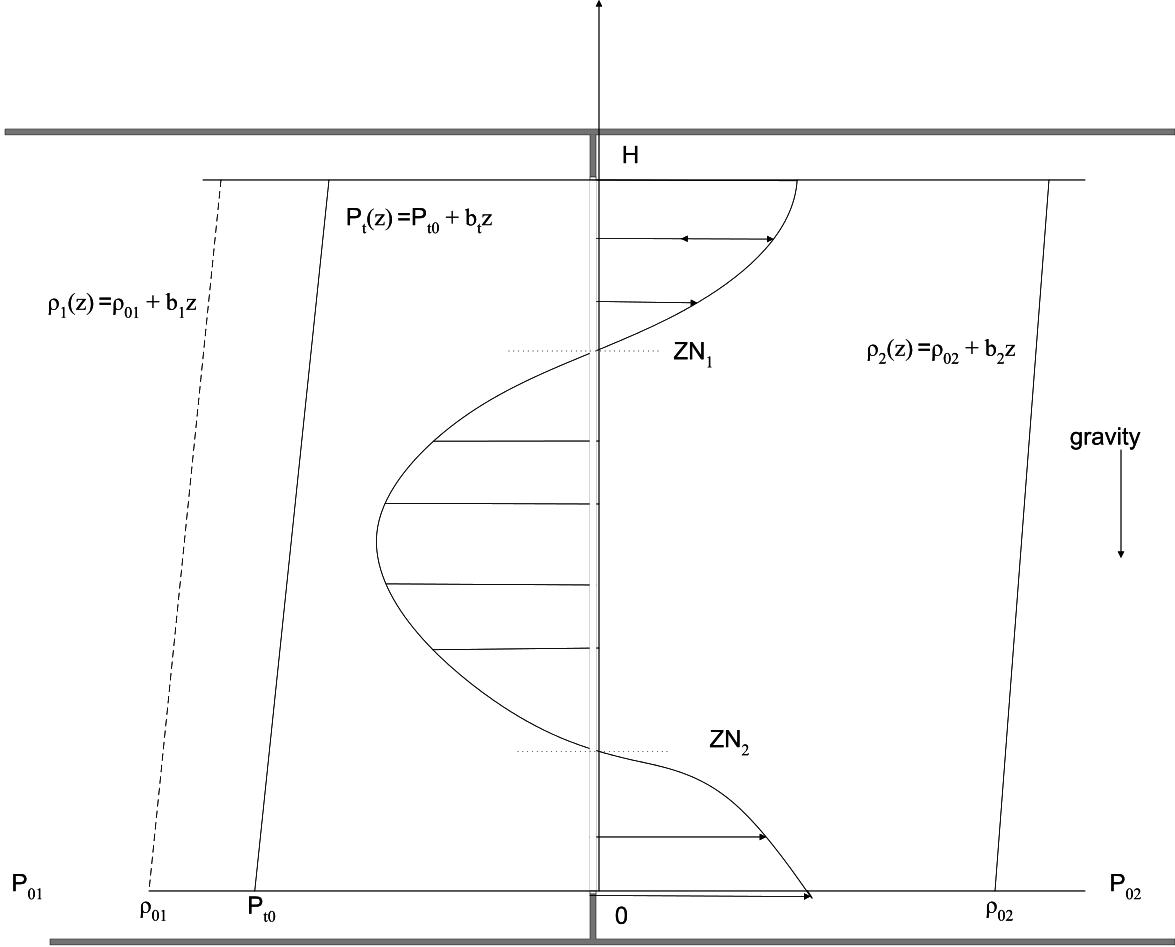
\includegraphics[width=0.9\linewidth, height=0.9\textheight, keepaspectratio=true]{media/image2691.svg.png}
\caption{The general problem of gravitational flow through a vertical opening \protect \label{fig:the-general-problem-of-gravitational-flow}}
\end{figure}

The schematic drawing of a possible air flow pattern through a detailed vertical opening (AirflowNetwork:Multizone:Component:DetailedOpening) is shown in Figure~\ref{fig:the-general-problem-of-gravitational-flow}. The equations used below are extracted from the COMIS Fundamentals manual (1990).

The air density is assumed to be a linear function of height:

\begin{equation}
{\rho_i}(z) = {\rho_{0i}} + {b_i}z
\end{equation}

The pressure difference is assumed to be linear and simulate the effect of turbulence:

\begin{equation}
\Delta P_t = P_{t0} + b_t z
\end{equation}

The reference pressures on each side are given at the bottom of the opening. By assuming the Bernoulli hypothesis on both sides, the pressure difference can be defined at any level of z as:

\begin{equation}
{P_1}(z) - {P_2}(z) = ({P_{01}} - {P_{02}}) - g\left[ {({\rho_{01}}z + {b_1}{z^2}/2) - ({\rho_{02}}z + {b_2}{z^2}/2)} \right] + ({P_{t0}} + {b_t}z)
\end{equation}

The velocity at any level z is given by

\begin{equation}
v(z) = \sqrt {2\frac{{{P_1}(z) - {P_2}(z)}}{\rho }}
\end{equation}

The locations of the two possible neutral planes are given by an equilibrium in pressure which leads to a zero velocity point. By assuming the left terms in the equation above to be zero, one may have:

\begin{equation}
g({b_1} - {b_2}){z^2}/2 + \left[ {g({\rho_{01}} - {\rho_{02}}) - {b_t}} \right]z + ( - {P_{01}} + {P_{02}} - {P_{t0}}) = 0
\end{equation}

This equation above can have two, one, or zero real solutions.~ The zero solution represents a one-way flow through the opening and may be expressed in the following equation:

\begin{equation}
\dot m = {C_d}\theta \int\limits_{z = 0}^{z = H} {\rho \nu (z)Wdz}
\end{equation}

The one real solution represents two-way (bi-directional) flow, which may be written in the following equations.

\begin{equation}
{\dot m_{0,z1}} = {C_d}\theta \int\limits_{z = 0}^{z = z1} {\rho \nu (z)Wdz}
\end{equation}

\begin{equation}
{\dot m_{z1,H}} = {C_d}\theta \int\limits_{z = z1}^{z = H} {\rho \nu (z)Wdz}
\end{equation}

The two real solutions represent three-way flow, which may be written in the following equations.

\begin{equation}
{\dot m_{z2,H}} = {C_d}\theta \int\limits_{z = z2}^{z = H} {\rho \nu (z)Wdz}
\end{equation}

\begin{equation}
{\dot m_{z1,z2}} = {C_d}\theta \int\limits_{z = z1}^{z = z2} {\rho \nu (z)Wdz}
\end{equation}

\begin{equation}
{\dot m_{z2,H}} = {C_d}\theta \int\limits_{z = z2}^{z = H} {\rho \nu (z)Wdz}
\end{equation}

where:

\begin{tabular}{lp{0.7\linewidth}}
\\
$C_d$ &= Discharge coefficient [dimensionless]\\
$\theta$ &= Area reduction factor [dimensionless]\\
$W$ &= Opening width [m]\\
\\
\end{tabular}

The discharge coefficient, opening width, opening height, and start height factor are modulated based on opening factors. A detailed description of opening factor calculations may be found in the Input Output Reference (Ref. AirflowNetwork:Multizone:Zone, AirflowNetwork:Multizone:Surface, and AirflowNetwork:Multizone:Component:DetailedOpening).

The above calculation procedure is used for a normal rectangular window. For a horizontally pivoted rectangular window, the calculation procedure is slightly different. A schematic drawing of a horizontally-pivoted window is shown in Figure~\ref{fig:schematic-drawing-of-a-horizontally-pivoted}.

\begin{figure}[hbtp] % fig 148
\centering
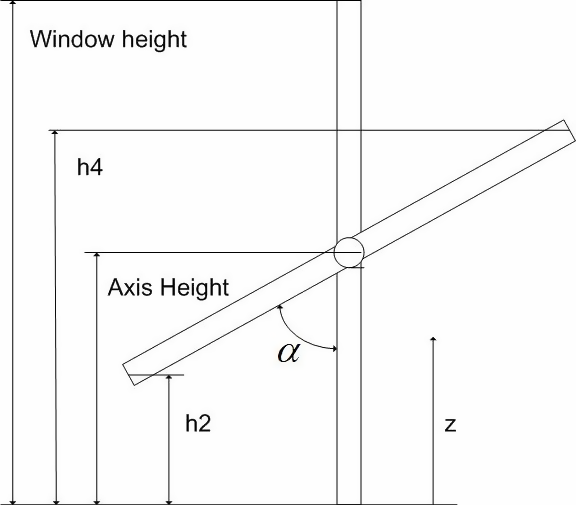
\includegraphics[width=0.9\linewidth, height=0.9\textheight, keepaspectratio=true]{media/image2703.png}
\caption{Schematic drawing of a horizontally-pivoted window \protect \label{fig:schematic-drawing-of-a-horizontally-pivoted}}
\end{figure}

The opening angle \(\alpha\) (0-90°) is linearly proportional to the window opening factor (0-1.0). An opening factor of 1.0 is equal to an opening angle of 90°. The heights in the pivoted area are expressed as:

\begin{equation}
h2 = AxisHeight(1 - \cos (\alpha ))
\end{equation}

\begin{equation}
h4 = AxisHeight + (WindowHeight - AxisHeight)\cos (\alpha )
\end{equation}

When z \textless{} h2 or z \textgreater{} h4, where z is the distance from the bottom of the window, the integration procedure is the same as the procedure for a normal rectangular window. When h2\textless{}z\textless{}h4, the window width W in the above equations is modified as:

\begin{equation}
W_{pivot} = \sqrt{\frac{1}{{\frac{1}{{{W^2}}} + \frac{1}{{{{(2(AxisHeight - z)\tan (\alpha ))}^2}}}}}}
\end{equation}

The mass flow rate in the pivoted area becomes:

\begin{equation}
{\dot m_{pivot}} = {C_d}\theta \int\limits_{z = h2}^{z = h4} {\rho \nu (z){W_{pivot}}dz}
\end{equation}

It should be pointed out that the discharge coefficient is modulated based on opening factors, while opening width, opening height, and start height factor do not apply for a horizontally-pivoted window. The actual window width and height are used to calculate airflows for a horizontally-pivoted window.

The schematic drawing of air flow patterns through a simple vertical opening (AirflowNetwork:Multizone:Component:SimpleOpening) is shown in Figure~\ref{fig:schematic-of-large-opening-and-associated}. The equations used below are available from Walton (1989).

\begin{figure}[hbtp] % fig 149
\centering
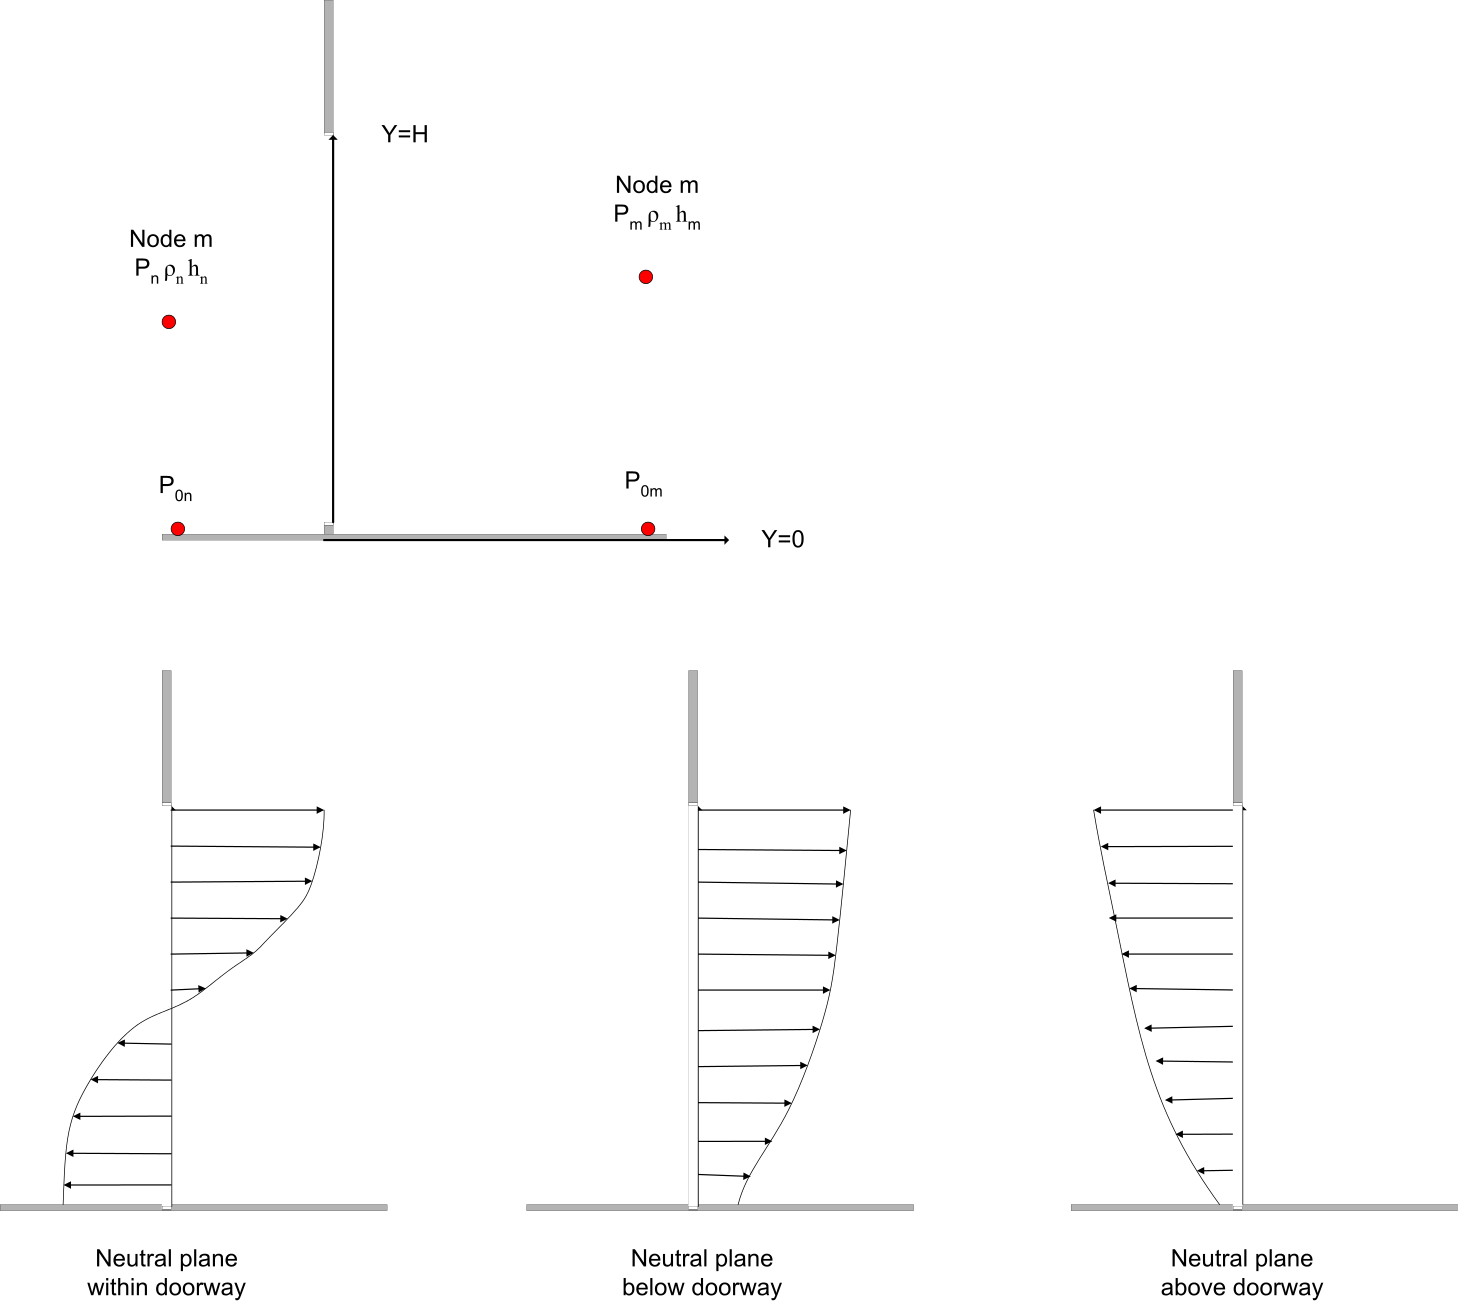
\includegraphics[width=0.9\linewidth, height=0.9\textheight, keepaspectratio=true]{media/image2708.svg.png}
\caption{Schematic of large opening and associated three flow patterns \protect \label{fig:schematic-of-large-opening-and-associated}}
\end{figure}

The air density for each node is assumed to be constant. The hydrostatic equation is used to relate pressures at various heights for each node:

\begin{equation}
Pn\left( y \right) = {P_{0n}} - {\rho_n}gy
\end{equation}

\begin{equation}
{P_m}(y) = {P_{0m}} - {\rho_m}gy
\end{equation}

where:

\begin{tabular}{lp{0.7\linewidth}}
\\
$P_{0n}, P_{0m}$ &= Pressure at nodes (zones) n and m at y = 0, the reference elevation of the opening [Pa] \\
$\rho_n, \rho_m$ &= Air densities of zones n and m [kg/m\(^{3}\)] \\
$P_n, P_m$ &= Reference pressures of zones n and m [Pa] \\
\\
\end{tabular}

It is assumed that the velocity of the airflow as a function of height is given by the orifice equation (Brown and Solvason 1962):

\begin{equation}
v(y) = {C_d}\sqrt {2\frac{{{P_n}(y) - {P_m}(y)}}{\rho }}
\end{equation}

where:

\begin{tabular}{lp{0.7\linewidth}}
\\
$C_d$ &= Discharge coefficient [dimensionless] \\
$\rho$ &= Density of the air going through the opening [kg/m\(^{3}\)] \\
\\
\end{tabular}

The neutral height, Y, where the velocity of the air is zero, may be calculated in the following equation:

\begin{equation}
Y = \frac{{{P_{on}} - {P_{0m}}}}{{g({\rho_n} - {\rho_m})}}\,\,\,\,\,\,\,\,or\,\,\,\,\,\,\,\frac{{{P_{om}} - {P_{0n}}}}{{g({\rho_m} - {\rho_n})}}
\end{equation}

When the neutral plane is within the opening (first pattern in Figure~\ref{fig:schematic-of-large-opening-and-associated}), two-way (bi-directional) flows occur. The total flow through a large opening is the sum of both flows.

\begin{equation}
{\dot m_{0,Y}} = {C_d}\theta \int\limits_{y = 0}^{y = Y} {\rho \nu (y)Wdy}
\end{equation}

\begin{equation}
{\dot m_{Y,H}} = {C_d}\theta \int\limits_{y = Y}^{y = H} {\rho \nu (y)Wdy}
\end{equation}

When the neutral plane is below or above the large opening (second and third pattern in Figure~\ref{fig:schematic-of-large-opening-and-associated}), one-way flow occurs.

\begin{equation}
{\dot m_{}} = {C_d}\theta \int\limits_{y = 0}^{y = H} {\rho \nu (y)Wdy}
\end{equation}

The opening width is modulated based on opening factors. A detailed description of opening factor calculations may be found in the Input Output Reference (Ref. AirflowNetwork:Multizone:Zone, AirflowNetwork:Multizone:Surface, and AirflowNetwork:Multizone:Component:DetailedOpening).

The above two objects are used to simulate airflows across large vertical openings. The simple opening component (AirflowNetwork:Multizone:Component:SimpleOpening) assumes the pressure difference across the opening is a function of height varied from opening bottom to top, so that two-way flow may be obtained if appropriate (Walton 1989). The Detailed Opening component (AirflowNetwork:Multizone:Component:DetailedOpening) assumes both the pressure difference across the opening and air density are a function of height, so that three-way flow may be obtained (COMIS 1990). If these opening models would be used for horizontal openings, the pressure difference across the opening and air density remain constant, so that only one-way flow is possible using the detailed and simple opening components which are meant for vertical or near-vertical openings. In reality, there are two-way flows (air recirculation) across a large horizontal opening caused by buoyancy due to temperature and pressure difference and forced flow driven by air pressure difference only. Therefore, a horizontal opening component (AirflowNetwork:Multizone:Component:HorizontalOpening) is available to simulate airflows across large horizontal openings with the possibility of two-way flow by combining forced and buoyancy airflows together.

The model for horizontal openings consists of forced airflow, buoyancy airflow, purge pressure and sloping plane. The model is mainly from a NIST report presented by Cooper (1989). The sloping plane (Bolmqvist and Sandberg 2004) portion of the model was added to allow for staircase simulations.

For simplicity, a two zone building (upper and lower zones) connected by a large horizontal opening is used to describe the model, as shown in Figure~\ref{fig:air-movements-across-a-horizontal-opening}. Forced and buoyancy airflows are described separately below.

\begin{figure}[hbtp] % fig 150
\centering
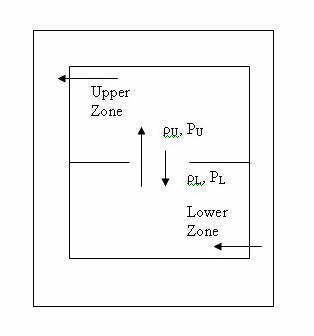
\includegraphics[width=0.9\linewidth, height=0.9\textheight, keepaspectratio=true]{media/image2716.png}
\caption{Air movements across a horizontal opening \protect \label{fig:air-movements-across-a-horizontal-opening}}
\end{figure}

\paragraph{Forced airflows}\label{forced-airflows}

The air mass flow rate is determined by the pressure difference across the opening. The relationship between pressure and airflow is the same as AIRNET for a component (see AirflowNetwork:Multizone:Component:SimpleOpening description above). Since the height of the opening is constant, the forced airflow is unidirectional. A positive value for pressure difference indicates flow direction is from the lower zone to the upper zone across the opening, while a negative value represents flow in the opposite direction. The following description addresses forced air mass flow rates and partial derivatives for three possible scenarios of pressure difference:

\textbf{Scenario 1}
\begin{gather}
P_L = P_U \\
\dot{m}_U = \dot{m}_L = 0
\end{gather}

where:

\begin{tabular}{lp{0.7\linewidth}}
\\
$P_L$ &= Air pressure in the lower zone [Pa] \\
$P_U$ &= Air pressure in the upper zone [Pa] \\
$\dot{m}_U$ &= Air mass flow rate from the lower zone to the upper zone driven by forced airflow pressure difference [kg/s]\\
$\dot{m}_L$ &= Air mass flow rate from the upper zone to the lower zone driven by forced airflow pressure difference [kg/s]\\
\\
\end{tabular}

\textbf{Scenario 2}

\begin{equation}
P_L > P_U
\end{equation}

\begin{equation}
\dot{m}_U = 0
\end{equation}

\begin{equation}
\dot{m}_L = \rho_L A C_d \left( {\frac{2\Delta P}{\rho_{ave}}} \right)^{0.5}
\end{equation}

\begin{equation}
\frac{\partial \dot{m}_L}{\partial {P_L}} = \rho_L A C_d \left( \frac{1}{2\Delta P \rho_{ave}} \right)^{0.5}
\end{equation}

where:

\begin{tabular}{lp{0.7\linewidth}}
\\
$\rho_L$ &= Air density in the lower zone [kg/m\(^{3}\)]\\
$A$ &= Opening area [m\(^{2}\)] \\
$C_d$ &= Discharge coefficient [Dimensionless]\\
$\rho_{ave}$ &= Average air density between the lower and upper zones [Pa] \\
$\Delta P$ &= Pressure difference P\(_{L}\) - P\(_{U}\) [Pa]\\
\\
\end{tabular}

\textbf{Scenario 3}

\begin{equation}
P_L < P_U
\end{equation}

\begin{equation}
\dot{m}_L = 0
\end{equation}

\begin{equation}
\dot{m}_U =  - {\rho_U}A{C_d}{\left( {\frac{{2\left| {\Delta P} \right|}}{{{\rho_{ave}}}}} \right)^{0.5}}
\end{equation}

\begin{equation}
\frac{{\partial \dot{m}_U}}{{\partial {P_L}}} = {\rho_U}A{C_d}{\left( {\frac{1}{{2\left| {\Delta P} \right|{\rho_{ave}}}}} \right)^{0.5}}
\end{equation}

where:

\begin{tabular}{lp{0.7\linewidth}}
\\
$\rho_U$ &= Air density in the upper zone [kg/m\(^{3}\)]\\
$A$ &= Opening area [m\(^{2}\)] \\
$C_{d}$ &= Discharge coefficient [Dimensionless] \\
$\rho_{ave}$ &= Average air density between the lower and upper zones [Pa] \\
$\Delta P$ &= Pressure difference P\(_{L}\) - P\(_{U}\) [Pa] \\
\\
\end{tabular}

\paragraph{Buoyancy airflows}\label{buoyancy-airflows}

Buoyancy flow only occurs when the air density in the upper zone is greater than the air density in the lower zone. The flow is bi-directional and the amount of upper flow is equal to the lower flow across the opening. The following discussion assumes the air density in the upper zone is greater than the air density in the lower zone. Otherwise, the buoyancy flow rate is equal to zero. It is also assumed that the maximum buoyancy flow occurs when the pressure difference across the opening due to forced airflows is zero. The maximum buoyancy flow may be expressed as a part of Cooper's model:

\begin{equation}
\dot{m}_{buo,\max} = {\rho_{ave}}\cdot0.055{\left( {\frac{{g\left| {\Delta \rho } \right|D_{_H}^5}}{{{\rho_{ave}}}}} \right)^{0.5}}
\end{equation}

where:

\begin{tabular}{lp{0.7\linewidth}}
\\
$\dot{m}_{buo,\max}$ &= Buoyancy mass flow rate at zero forced airflow pressure difference [kg/s]\\
$g$ &= Gravity acceleration [m/s\(^{2}\)]\\
$D_H$ &= Hydraulic diameter [m] \\
$\rho_{ave}$ &= Average air density between the lower and upper zones [kg/m\(^{3}\)]\\
$\Delta \rho$ &= Density difference between the lower and upper zones [kg/m\(^{3}\)]\\
\\
\end{tabular}

\paragraph{Combined airflows}\label{combined-airflows}

When forced and buoyancy flows co-exist, it is possible to have either unidirectional or bi-directional flows. For example, when the upward force due to pressure difference is greater than the buoyancy force (downward), unidirectional flow occurs. Bi-directional flow only occurs when the upward imposed force is less than the buoyancy force. The critical pressure between unidirectional and bi-directional flows is called the purge pressure (Tan and Jaluria 1992). The purge pressure is a function of opening geometry and the buoyancy force (ΔP/(gΔρD\(_{H}\))) and may be expressed as (Cooper 1998):

\begin{equation}
\Delta {P_{Flood}} = \left| {C_{Shape}^2\frac{{g\Delta \rho D_H^5}}{{2{A^2}}}} \right|
\end{equation}

where:

\begin{tabular}{lp{0.7\linewidth}}
\\
$\Delta P_{Flood}$ &= Purging pressure [Pa]\\
$g$ &= Gravity acceleration [m/s\(^{2}\)]\\
$D_H$ &= Hydraulic diameter [m]\\
$A$ &= Opening area [m\(^{2}\)]\\
$\Delta \rho$ &= Density difference between the lower and upper zones [kg/m\(^{3}\)]\\
$C_{Shape}$ &= Shape factor [dimensionless]\\
\\
\end{tabular}

\begin{equation}
C_{Shape} = \left\{ \begin{array}{l}0.754\;\;\;{\rm{for}}\;{\rm{a}}\;{\rm{circle}}\;{\rm{opening}}\\0.942(w/D)\;{\rm{for}}\;{\rm{a}}\;{\rm{rectangle}}\;{\rm{opening}}\end{array} \right\}
\end{equation}

where:

\begin{tabular}{lp{0.7\linewidth}}
\\
$w$ &= Opening width [m]\\
$D$ &= Opening depth [m]\\
\\
\end{tabular}

As mentioned above, when the air pressure difference between two zones is zero there is the maximum bi-directional flow due to the buoyancy force. When the pressure difference increases from 0 and is less than \textbar{}$\Delta P_{Flood}$\textbar{}, there is some bi-directional flow across the opening, but less than the maximum flow. If the pressure difference keeps increasing and exceeds \textbar{}$\Delta P_{Flood}$\textbar{}, there is no bi-directional flow.~ Cooper's model assumes the buoyancy flow varies linearly with pressure difference.

\begin{equation}
\dot{m}_{buo} = \left\{ \begin{array}{l}{\dot{m}_{buo,\max }}\cdot\left( {1 - \frac{{\left| {\Delta P} \right|}}{{\left| {\Delta {P_{Flood}}} \right|}}} \right)\;\,\,\mbox{If}\;\Delta \rho  > 0\;\mbox{and}\;\frac{{\left| {\Delta P} \right|}}{{\left| {\Delta {P_{Flood}}} \right|}} < 1\\0\;\,\,\,\mbox{Otherwise}\end{array} \right\}
\end{equation}

The total air flow across the opening is based on superposition of the forced and buoyancy flows, and may be expressed for three different pressure difference scenarios as follows:

\textbf{a. $P_L = P_U$}

\begin{equation}
\dot{m}_U = \dot{m}_{buo}
\end{equation}

\begin{equation}
\dot{m}_L = \dot{m}_{buo}
\end{equation}

\begin{equation}
\frac{\partial \dot{m}_L}{\partial P_L} = 0
\end{equation}

\textbf{b. $P_L > P_U$}

\begin{equation}
\dot{m}_U = \dot{m}_{buo}
\end{equation}

\begin{equation}
\dot{m}_L = \rho_L A C_d \left( \frac{2 \Delta P}{\rho_{ave}} \right)^{0.5} + \dot{m}_{buo}
\end{equation}

\begin{equation}
\frac{\partial \dot{m}_L}{\partial P_L} = \rho_L A C_d \left( \frac{1}{2\Delta P \rho_{ave}} \right )^{0.5} - \frac{\dot{m}_{buo,max}}{|\Delta P_{Flood}|}
\end{equation}

where:

\begin{tabular}{lp{0.7\linewidth}}
\\
$\rho_L$ &= Air density in the lower zone [kg/m\(^{3}\)]\\
$A$ &= Opening area [m\(^{2}\)]\\
$C_d$ &= Discharge coefficient [dimensionless]\\
$Ρ_{ave}$ &= Average air density between the lower and upper zones [Pa]\\
$\Delta P$ &= Pressure difference P\(_{L}\) - P\(_{U}\) [Pa]\\
\\
\end{tabular}

\textbf{c.  $P_L < P_U$}

\begin{equation}
\dot{m}_L = \dot{m}_{buo}
\end{equation}

\begin{equation}
\dot{m}_U =  - \rho_U A C_d \left( \frac{2\left| \Delta P \right|}{\rho_{ave}} \right)^{0.5} + \dot{m}_{buo}
\end{equation}

\begin{equation}
\frac{\partial \dot{m}_U}{\partial P_L} = \rho_U A C_d \left( \frac{1}{2 \left| \Delta P \right| \rho_{ave}} \right)^{0.5} + \frac{\dot{m}_{buo,max}}{\left| \Delta P_{Flood} \right|}
\end{equation}

\paragraph{Sloping Plane}\label{sloping-plane}

\begin{figure}[hbtp] % fig 151
\centering
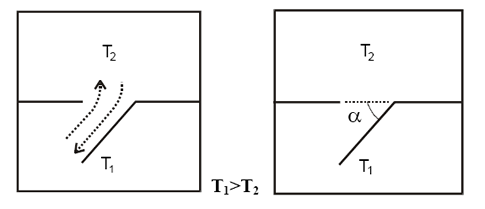
\includegraphics[width=0.9\linewidth, height=0.9\textheight, keepaspectratio=true]{media/image2741.png}
\caption{A Staircase is attached to the horizontal opening. \protect \label{fig:a-staircase-is-attached-to-the-horizontal}}
\end{figure}

When a staircase is introduced as shown in Figure~\ref{fig:a-staircase-is-attached-to-the-horizontal}, the effective opening area will be used to replace A (opening area) in the above equations. The effective area may be estimated as (Bolmqvist and Sandberg 2004):

\begin{equation}
A_{eff} = A\sin \alpha (1 + \cos \alpha )
\end{equation}

where:

\begin{tabular}{lp{0.7\linewidth}}
\\
$A_{eff}$ &= Effective area of horizontal opening [m\(^{2}\)]\\
$A$ &= Area of horizontal opening [m\(^{2}\)] \\
$\alpha$ &= Angle between the stair plane and horizontal opening plane [degrees]\\
\\
\end{tabular}

Note: the hydraulic diameter calculation is based on the effective opening area, while the opening depth remains the same.

Figure~\ref{fig:flow-rates-at-different-pressure-differences} demonstrates possible forced and buoyancy flow rates at different ratios of pressure difference to purging pressure across a horizontal opening when the upper zone air density is greater than the lower zone air density. The pressure difference is the lower zone pressure minus the upper zone pressure. Otherwise, the buoyancy flow is zero. In addition, when the absolute ratio is above 1, the buoyancy flow is also zero. The following table provides a brief description for the legend listed in Figure~\ref{fig:flow-rates-at-different-pressure-differences}.

% table 49
\begin{longtable}[c]{p{1.5in}p{4.5in}}
\caption{Legend Description \label{table:legend-description}} \tabularnewline
\toprule 
Legend & Description \tabularnewline
\midrule
\endfirsthead

\caption[]{Legend Description} \tabularnewline
\toprule 
Legend & Description \tabularnewline
\midrule
\endhead

Forced downward & Forced flow rate from upper to lower at P  -P    <  0 \tabularnewline
Forced upward & Forced flow rate from lower to upper at P  -P    >  0 \tabularnewline
Buoyancy upward & Total upward flow rate due to buoyancy only at P  -P    <  0 \tabularnewline
Buoyancy downward & Total downward flow rate due to buoyancy only at P  -P    >  0 \tabularnewline
Combined downward & Total downward flow at P  -P    <  0 (Forced downward + buoyancy upward) \tabularnewline
Combined upward & Total upward flow at P  -P    >  0 (Forced upward + buoyancy downward) \tabularnewline
\bottomrule
\end{longtable}

\begin{figure}[hbtp] % fig 152
\centering
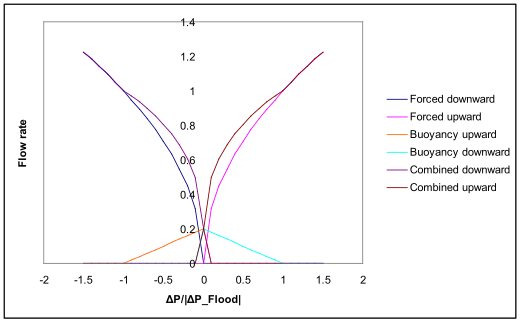
\includegraphics[width=0.9\linewidth, height=0.9\textheight, keepaspectratio=true]{media/image2743.svg.png}
\caption{Flow rates at different pressure differences \protect \label{fig:flow-rates-at-different-pressure-differences}}
\end{figure}

\subsubsection{Wind pressure calculations}\label{wind-pressure-calculations}

The wind pressure is determined by Bernoulli's equation, assuming no height change or pressure losses:

\begin{equation}
p_w = C_p \rho \frac{V_{ref}^2}{2}
\end{equation}

where:

\begin{tabular}{lp{0.7\linewidth}}
\\
$p_w$ &= Wind surface pressure relative to static pressure in undisturbed flow [Pa]\\
$\rho$ &= Air density [kg/m\(^{3}\)]\\
$V_{ref}$ &= Reference wind speed at local height [m/s]\\
$C_p$ &= Wind surface pressure coefficient [dimensionless]\\
\\
\end{tabular}

$V_{ref}$ may be expressed as (Ref, Local Wind Speed Calculations)

\begin{equation}
V_{ref} = V_{met} \left( \frac{\delta_{met}}{z_{met}} \right)^{\alpha_{met}}\left( \frac{z}{\delta} \right)^\alpha
\end{equation}

$C_p$ is a function of location on the building envelope and wind direction. When Wind Pressure Coefficient Type = ``INPUT'', the $C_p$ values are explicitly defined in the input for AirflowNetwork:Multizone:Wind Pressure Coefficient Values. When Wind Pressure Coefficient Type = ``AVERAGE-SURFACE CALCULATION'' and the building shape is rectangular, the program uses the following equations to calculate wind pressure coefficient ($C_p$) values for different wind directions. For a low rise building, the normalized surface pressure coefficient may be written as (Swami and Chandra 1988):

\begin{equation}
C_{p,n} = 0.6 \cdot \ln \left[ \begin{array}{l}1.248 - 0.703\sin (\alpha /2) - 1.175{\sin ^2}(\alpha ) + 0.131{\sin ^3}(2\alpha G)\\ + \,0.769\cos (\alpha /2) + 0.07{G^2}{\sin ^2}(\alpha /2) + 0.717{\cos ^2}(\alpha /2)\end{array} \right]
\end{equation}

where:

\begin{tabular}{lp{0.7\linewidth}}
\\
$C_{p,n}$ &= $C_p$ value at a given angle between wind direction and the outward normal of the surface under consideration [dimensionless]\\
$\alpha$ &= Angle between wind direction and outward normal of wall under consideration [deg]\\
$G$ &= Natural log of the ratio of the width of the wall under consideration to the width of the adjacent wall [dimensionless]\\
$n$ &= Index of incident angle at 30-degree increments\\
\\
\end{tabular}

For walls of a high rise building, a two-dimensional array of surface-averaged wind pressure coefficients is generated based on wind incident angle and side ratio. The wind pressure coefficients are provided in 2001 ASHRAE Fundamentals Handbook, p.~16.5, Fig. 7, ``Surface Averaged Wall Pressure Coefficients for Tall Buildings''. The original work was performed by Atkins et al. (1979). The incident angle has an increment of 30 degrees. The side ratio values are 0.25, 1.0, and 4.0. For a given incident angle and building aspect ratio, the program uses linear interpolation to calculate the corresponding wind pressure coefficient $C_{p,n}$.

For the roof of a high rise building, a two-dimensional array of surface-averaged wind pressure coefficients is also generated based on wind incident angle and side ratio. The wind pressure coefficients are provided in 2001 ASHRAE Fundamentals Handbook, p.~16.6, Fig. 9, ``Surface Averaged Roof Pressure Coefficients for Tall Buildings''. The original work was performed by Holmes (1986). The incident angle has an increment of 30 degrees. The side ratio values are 0.25, 1.0, and 4.0. At a given wind incident angle and building aspect ratio, the program uses linear interpolation to calculate the corresponding wind pressure coefficient $C_{p,n}$.

The wind surface pressure at the given incident angle can be calculated by combining the above two equations:

\begin{equation}
p_{w,n} = C_{p,n}\rho \frac{V_{ref}^2}{2}
\end{equation}

\subsubsection{Solution method}\label{solution-method}

Based on the relationship between airflow rate and pressure drop for each component, a system of equations for all components can be assembled together in an n x n square matrix, where n is the number of nodes. Newton's method is used to iteratively solve for the air pressure at each node. A new estimated vector for all node pressures, \{P\}*, is computed from the current estimated vector of node pressures, \{P\}, by:

\begin{equation}
{\left\{ P \right\}^*} = \left\{ P \right\} - \left\{ C \right\}
\end{equation}

where the correction vector, \{C\}, is computed by the matrix relationship:

\begin{equation}
\left[ J \right]\left\{ C \right\} = \left\{ B \right\}
\end{equation}

\{B\} is a column vector with each component given by:

\begin{equation}
B_n = \sum_{i} \dot{m}_i
\end{equation}

where $n$ is the node number and $i$ indicates all flow paths connecting node $n$ to other nodes, and [J] is the square Jacobian matrix whose elements are given by:

\begin{equation}
J_{n,m} = \sum_{i} \frac{\partial \dot{m}}{\partial P_m}
\end{equation}

\subsubsection{Convergence acceleration}\label{convergence-acceleration}

The convergence tolerance is used to check the sum of the mass flow rates by applying mass conservation. The convergence acceleration equation shown below is used to correct the node pressures to more rapidly obtain a solution. By assuming a constant ratio of correction values from one iteration to the next, the following method is applied:

\begin{equation}
{P_n}^* = P_n - C_n/(1 - r)
\end{equation}

where:

\begin{tabular}{lp{0.7\linewidth}}
\\
$r$ &= the ratio of $C_n$ for the current iteration to its value for the previous iteration [dimensionless]\\
$C_n$ &= Correction value at the n-th node [Pa]\\
$P_n$ &= Estimated pressure at the n-th node [Pa]\\
$P_n^*$ &= Corrected pressure at the n-th node used in the next iteration [Pa]\\
\\
\end{tabular}

This method is similar to a Steffensen iteration (Conte and de Boor 1972) which is used as a fixed-point iteration method for individual nonlinear equations.

The iteration correction method presented in the above equation gives a variable factor. When the solution is close to convergence, the solution method converges quadratically. By limiting cases where the value of r is less than some value, such as -0.5, the solution will not interfere with the rapid convergence. It has not been proven that the convergence acceleration equation will always lead to convergence, but it can be shown that it will not prevent convergence. Newton's method converges when the estimated solution values are within some distance, called the radius of convergence, or the correct solution. Applying the convergence acceleration equation when -1 \textless{} r \textless{}0, will cause a smaller correction than Newton's method, which therefore, can not force the iterations outside the radius of convergence. When r\textless{}-1, the solution diverges in an oscillatory fashion. When r\textgreater{}1, the solution also diverges, but in a nonoscillatory manner. For 0\textless{}r\textless{}1, the solution is approached from one direction. In all three cases, the convergence acceleration equation applies as long as r is truly constant over several iterations. However, for the last case, this involves a true extrapolation of correction factor which is very sensitive to the accuracy of r. This is most extreme for the case of r = 1, which would cause an infinite correction.

\subsection{Node Temperature Calculations}\label{node-temperature-calculations}

\subsubsection{General}

A brief description of the air node temperature calculation is given below. A detailed description can be found in the work of Swami et al. (1992). The following equation is used to calculate temperature distribution across a duct element at the given airflow rate and inlet air temperature:

\begin{equation}
\dot{m} C_p \frac{dT}{dx} = UP(T_\infty  - T)
\end{equation}

where:

\begin{tabular}{lp{0.7\linewidth}}
\\
$C_p$ &= Specific heat of airflow [J/kg-K]\\
$\dot{m}$ &= Airflow rate [kg/s]\\
$P$ &= Perimeter of a duct element [m]\\
$T$ &= Temperature as a field variable [°C]\\
$T_\infty$ &= Temperature of air surrounding the duct element [°C]\\
$U$ &= Overall heat transfer coefficient [W/m\(^{2}\)-K]\\
\\
\end{tabular}

\begin{equation}
U = \frac{1}{{\frac{1}{{{h_i}}} + \frac{1}{{{h_o}}} + \sum {\frac{{{t_j}}}{{{k_j}}}} }}
\end{equation}

\begin{tabular}{lp{0.7\linewidth}}
\\
$h_i$ &= Inside heat transfer coefficient [W/m\(^{2}\)-K]\\
$h_o$ &= Outside heat transfer coefficient [W/m\(^{2}\)-K]\\
$t_j$ &= Thickness at j-th layer [m]\\
$k_j$ &= Thermal conductivity at j-th layer [W/m-K]\\
\\
\end{tabular}

The outlet air temperature at the end of the duct (x = L) is:

\begin{equation}
T_o = T_\infty + (T_i - T_\infty) \cdot \exp \left(- \frac{UA}{\dot{m} C_p} \right)
\end{equation}

where:

\begin{tabular}{lp{0.7\linewidth}}
\\
$T_i$ &= Inlet air temperature [°C]\\
$T_o$ &= Outlet air temperature [°C]\\
$T_\infty$ &= Temperature of air surrounding the duct element [°C]\\
$A$ &= Surface area (Perimeter * Length) [m\(^{2}\)]\\
\\
\end{tabular}

The heat transfer by convection to ambient, $Q$, is:

\begin{equation}
Q = \dot{m} {C_p}(T_\infty- T_i)\left[1 - \exp \left( - \frac{UA}{\dot{m} C_p} \right) \right]
\end{equation}

The outlet air temperature can be calculated using the above equation at the given inlet air temperature. Since the inlet temperature at one linkage is the outlet temperature for the connected linkage, the outlet air temperatures at all nodes are solved simultaneously. A square linear system assembled by the AirflowNetwork model is expressed below:

\begin{equation}
\{ M\} [T] = [B]
\end{equation}

where:

\begin{tabular}{lp{0.7\linewidth}}
\\
$\{M\}$ &= Airflow matrix\\
$[T]$ &= Temperature vector\\
$[B]$ &= Given boundary conditions\\
\\
\end{tabular}

The zone air temperatures and primary air loop component (fan and coils) outlet conditions are used as prescribed conditions in the AirflowNetwork model. In addition, the temperature difference across zone loop components (terminal units) is held constant during the calculations. For example, thermal zone temperatures calculated during the previous system time step are used as prescribed temperatures when calculating all other node temperatures. The zone air temperature is assumed constant (prescribed) throughout the AirflowNetwork iterative solution. The fan and coil outlet air temperatures, and terminal unit temperature differences are assumed constant within an AirflowNetwork iteration. The sensible heat gains calculated during the AirflowNetwork solution are then used to predict a new zone air temperature.

\subsubsection{Duct Radiation}

The duct-surface user-defined view factors object defines the view factor from the duct to the zone surfaces. Because the view factors, duct surface area, and temperatures are known, the heat gain to the duct can be directly calculated and applied to the duct air heat balance to determine the outlet temperature. The duct heat gain is then treated as a direct heat loss from each participating surface. Once the heat loss to the duct for each surface is calculated, the surface temperatures are adjusted to maintain the surface energy balance.

Radiation is treated as point loads heat source/sink on the zone surfaces and the duct.  These point loads will be added or subtracted using the same implementation strategy as the convective load for the ducts to the zone air.  The radiative rate of energy transfer between the duct (d) and a given surface (s) for two grey surfaces can be written as shown below.


\begin{equation}
\dot{Q}_{d\rightarrow s} = \frac{\sigma (T^4_d - T^4_s)}{\frac{1 - \epsilon_d}{f_e A_d \epsilon_d} + \frac{1}{f_e A_d F_{d\rightarrow s}}+\frac{1 - \epsilon_s}{A_s \epsilon_s}}
\end{equation}

where:

\begin{tabular}{lp{0.7\linewidth}}
\\
$\sigma$ &= Steffan-Boltzmann constant [W/m\(^{2}\)-K\(^{4}\)] \\
$T_d$ &= Duct surface temperature [C] \\
$T_s$ &= Zone surface temperature [C] \\ 
$\epsilon_d$ &= Duct grey body emissivity [-] \\
$\epsilon_s$ &= Zone surface grey body emissivity [-] \\
$A_d$ &= Duct surface area [m\(^{2}\)] \\
$A_s$ &= Zone surface area [m\(^{2}\)] \\
$f_e$ &= Duct exposure fraction [-] \\
$F_{d\rightarrow s}$ &= Duct-to-surface view factor \\
\\
\end{tabular}

\subsection{Node Humidity Ratio Calculations}\label{node-humidity-ratio-calculations}

A brief description of the air node humidity ratio calculation is given below. A detailed description can found in the work of Swami et al. (1992). The following equation is used to calculate humidity ratio distribution across a duct element at the given airflow rate and inlet air humidity ratio:

\begin{equation}
\dot{m} \frac{dW}{dx} = U_m P(W_\infty - W)
\end{equation}

where:

\begin{tabular}{lp{0.7\linewidth}}
\\
$\dot{m}$ &= Airflow rate [kg/s]\\
$P$ &= Perimeter of a duct element [m]\\
$W$ &= Humidity ratio [kg/kg]\\
$W_\infty$ &= Humidity ratio of air surrounding the duct element [kg/kg]\\
$U_m$ &= Overall moisture transfer coefficient [kg/m\(^{2}\)-s]\\
\\
\end{tabular}

\begin{equation}
U_m = \frac{1}{\frac{1}{h_{m,i}} + \frac{1}{h_{m,o}} + \sum {\frac{t_j}{D_j}} }
\end{equation}

\begin{tabular}{lp{0.7\linewidth}}
\\
$h_{m,i}$ &= Inside moisture transfer coefficient [kg/m\(^{2}\)-s]\\
$h_{m,o}$ &= Outside moisture transfer coefficient [kg/m\(^{2}\)-s]\\
$t_j$ &= Thickness at j-th layer [m]\\
$D_j$ &= Moisture diffusivity at j-th layer [kg/m-s]\\
\\
\end{tabular}

The outlet air humidity ratio at the end of the duct (x = L) is:

\begin{equation}
W_o = W_\infty + (W_i - W_\infty) \cdot \exp \left(- \frac{U_m A}{\dot{m}} \right)
\end{equation}

where:

\begin{tabular}{lp{0.7\linewidth}}
\\
$W_i$ &= Inlet air humidity ratio [kg/kg]\\
$W_o$ &= Outlet air humidity ratio [kg/kg]\\
$A$ &= Surface area (Perimeter * Length) [m\(^{2}\)]\\
\\
\end{tabular}

The moisture transfer by convection to ambient, \emph{Q\(_{m}\)}, is

\begin{equation}
Q_m = \dot{m} \cdot (W_\infty - W_i)\left[ 1 - \exp \left(- \frac{U_m A}{\dot{m}} \right) \right]
\end{equation}

The outlet air humidity ratio can be calculated using the above equation at the given inlet air humidity ratio. Since the inlet humidity ratio at one linkage is the outlet humidity ratio for the connected linkage, the outlet air humidity ratio at all nodes are solved simultaneously. A square linear system assembled by the AirflowNetwork model is expressed below:

\begin{equation}
\{M_m\} [W] = [B_m]
\end{equation}

where:

\begin{tabular}{lp{0.7\linewidth}}
\\
$\{M_m\}$ &= Airflow matrix\\
$[W]$ &= Humidity ratio vector\\
$[B_m]$ &= Given boundary conditions\\
\\
\end{tabular}

The zone air humidity ratios and primary air loop component (fan and coils) outlet conditions are used as prescribed conditions in the AirflowNetwork model. For example, thermal zone humidity ratios calculated during the previous system time step are used as prescribed humidity ratios when calculating all other node humidity ratios. The zone air humidity ratio is assumed constant (prescribed) throughout the AirflowNetwork iterative solution. The coil outlet air humidity ratio is assumed constant within an AirflowNetwork iteration. The latent heat gains calculated during the AirflowNetwork solution are then used to predict a new zone air humidity ratio.

\subsection{Sensible and Latent Load Calculations}\label{sensible-and-latent-load-calculations}

The zone sensible and latent loads calculated in the AirflowNetwork model consist of multizone, duct conduction and leakage. In addition, the impact of infiltration and mixing is accounted for in this calculation. The multizone load only includes incoming airflows from outside (infiltration) and other adjacent zones (mixing) with and without forced-air fan operation. It is divided into two terms: variable and constant. The constant term is the sum of the mass flow rate multiplied by the specific heat for both infiltration and mixing. The variable term includes the impact of zone and outdoor air temperature. Each of these terms is used in the zone energy balance equation. The sensible load items from the multizone load calculations may be written as follows:

\begin{equation}
MCP_{airflow} = \dot{m}_{inf} {C_p} + \sum \left( {\dot{m}_{mix} C_p} \right)
\end{equation}

\begin{equation}
MCPT_{airflow} = \dot{m}_{inf} C_p T_{amb} + \sum \left( \dot{m}_{mix} C_p T_{zone} \right)
\end{equation}

where:

\begin{tabular}{lp{0.7\linewidth}}
\\
$MCP_{airflow}$ &= Sum of air mass flow rate multiplied by specific heat for infiltration and mixing [W/K]\\
$MCPT_{airflow}$ &= Sum of air mass flow rate multiplied by specific heat and temperature for infiltration and mixing [W]\\
$\dot{m}_{inf}$ &= Incoming air mass flow rate from outdoors [kg/s]\\
$\dot{m}_{mix}$ &= Incoming air mass flow rate from adjacent zones [kg/s]\\
$T_{amb}$ &= Outdoor air dry-bulb temperature [°C]\\
$T_{zone}$ &= Adjacent zone air temperature [°C]\\
\\
\end{tabular}

The latent load items from multizone load calculations may be written as follows:

\begin{equation}
M_{airflow} = \dot{m}_{inf} + \sum \dot{m}_{mix}
\end{equation}

\begin{equation}
MW_{airflow} = \dot{m}_{inf} W_{amb} + \sum \dot{m}_{mix} W_{zone}
\end{equation}

where:

\begin{tabular}{lp{0.7\linewidth}}
\\
$M_{airflow}$ &= Sum of air mass flow rates for infiltration and mixing [kg/s]\\
$MW_{airflow}$ &= Sum of air mass flow rate multiplied by humidity ratio for infiltration and mixing [kg/s]\\
$\dot{m}_{inf}$ &= Incoming air mass flow rate from outdoors [kg/s]\\
$\dot{m}_{mix}$ &= Incoming air mass flow rate from adjacent zones [kg/s]\\
$W_{amb}$ &= Outdoor air humidity ratio [kg/kg]\\
$W_{zone}$ &= Adjacent zone air humidity ratio [kg/kg]\\
\\
\end{tabular}

The air distribution system (ADS) loads due to duct conduction and leakage depend on the air distribution system component (e.g., duct) location. The air distribution system sensible and latent loads are calculated for each zone as follows:

\begin{equation}
Q_{ADS,i} = \sum_{j} Q_{cond(i,j)} + \sum_{j} Q_{leak(i,j)}
\end{equation}

\begin{equation}
Q_{ADS,m,i} = \sum_{j} Q_{cond,m(i,j)} + \sum_{j} Q_{leak,m(i,j)}
\end{equation}

where:

\begin{tabular}{lp{0.7\linewidth}}
\\
$Q_{ADS,i}$ &= Total sensible load in the i-th zone due to ADS losses [W]\\
$Q_{cond(ij)}$ &= Duct wall conduction loss at the j-th duct located in the i-th zone [W]\\
$Q_{leak(ij)}$ &= Sensible supply leak loss at the j-th linkage located in the i-th zone [W]\\
$Q_{ADS,m,i}$ &= Total latent load in the i-th zone due to ADS losses [kg/s]\\
$Q_{cond,m(ij)}$ &= Duct wall vapor diffusion loss at the j-th duct located in the i-th zone [kg/s]\\
$Q_{leak,m(ij)}$ &= Latent supply leak loss at the j-th linkage located in the i-th zone [kg/s]\\
\\
\end{tabular}

\subsection{Impacts of Supply Air Constant Volume Fan Control on Load: Cycling vs.~Continuous}\label{impacts-of-supply-air-constant-volume-fan-control-on-load-cycling-vs.continuous}

The AirflowNetwork model currently allows two types of constant volume fans: Fan:ConstantVolume and Fan:OnOff. The Fan:ConstantVolume object has only one type of supply air fan operation mode: continuous fan, cycling compressor (ContinuousFanWithCyclingCompressor). However, the Fan:OnOff has two types of supply air fan operation modes: cycling fan, cycling compressor (CyclingFanAndCompressor) or continuous fan, cycling compressor (ContinuousFanWithCyclingCompressor). The CyclingFanAndCompressor operation mode is frequently referred to as ``AUTO fan'', where the compressor(s) and supply air fan operate in unison to meet the zone heating or cooling load, and cycle off together when the heating or cooling load has been met. The ContinuousFanWithCyclingCompressor operation mode is often referred to as ``fan ON'', where the compressor(s) cycle on and off to meet the zone heating or cooling load but the supply air fan operates continuously regardless of compressor operation. The supply air fan operation mode is specified in an HVAC system object based on a given fan operation mode schedule (e.g., AirLoopHVAC:UnitaryHeatCool object).

The determination of the zone sensible and latent loads caused by multizone airflows and forced air distribution system operation is dependent on the supply air fan operation mode (see Sensible and Latent Load Calculations section above). The zone loads calculated by the AirflowNetwork model are added to zone sensible and latent balances in the ZonePredictorCorrector module to calculate zone air temperatures and humidity ratios (see Integration of the AirflowNetwork Model section below). For the case of continuous fan/cycling compressor, the zone loads during forced air distribution system operation are calculated with the system design air mass flow rate without modification, since the system air node conditions (temperature and humidity) reflect the average values for the time step considering the coil/fan on and off periods during the time step.

For the case of cycling fan/cycling compressor, where the forced air distribution system can operate for a portion of the simulation time step, the airflows are determined based on the air distribution system part-load ratio (ratio of the average air mass flow rate for the time step divided by the design air mass flow rate). The \textbf{airflows} for the AirflowNetwork:Distribution:Linkage objects are reported during the air distribution system on cycle, since no airflow is assumed during the system off cycle. The \textbf{airflows} for the AirflowNetwork:Multizone:Surface objects are weighted by the air distribution system part-load ratio. The \textbf{zone loads} are the sum of energy losses during both the air distribution system on and off cycle at each system time step. The energy losses when the air distribution system is on are calculated using the system ``on'' air flow rate multiplied by the air distribution system run time fraction. The energy losses when the air distribution system is off are obtained from the multizone airflow calculations (without forced air through the air distribution system) and these losses are multiplied by (1.0 - system run time fraction), assuming no airflows through the air distribution system when the fan is off. The formulas used to calculate airflows and zone loads are given below:

Airflow

\begin{tabular}{lp{0.7\linewidth}}
\\
Airflow = &Airflow~during~ADS~on~cycle~*~ADS~Part-load~ratio~+~Airflow~during~ADS~off~cycle~*~(1.0~--~ADS~Part-load~ratio)\\
\\
\end{tabular}

where:

\begin{tabular}{lp{0.7\linewidth}}
\\
$ADS$ &= Air Distribution System\\
\\
\end{tabular}

Zone load

\begin{tabular}{lp{0.7\linewidth}}
\\
System run time fraction = &Maximum~run~time~fraction~of~coils~and~fans~in~the~air~distribution~system\\
\\
Zone energy losses ~~~~~~~~= &Zone~energy~loss~during~ADS~on~cycle~*~System~run~time~fraction~+~Zone~energy~loss~during~ADS~off~cycle~*~(1.0~-~System~run~time~fraction)\\
\\
\end{tabular}

The calculation of loads due to multizone airflow, without forced air distribution system operation, is performed when the HVAC system is first simulated during a simulation time step (FirstHVACIteration = True). The calculation of loads due to air distribution system operation is performed on subsequent iterations within the same simulation time step when the mass flow rate at the supply air fan inlet is greater than 0.0 (and FirstHVACIteration = False).

\subsection{Airflow Calculation Procedure using A Supply Variable Air Volume Fan}\label{airflow-calculation-procedure-using-a-supply-variable-air-volume-fan}

The AirflowNetwork model currently also allows a variable air volume fan type as Fan:VariableVolume. The allowed terminal type is AirTerminal:SingleDuct:VAV:Reheat only. Other types of terminals will be added later.

In general, the supply fan air flow rate in a VAV central system is determined by a sum of terminal flow rates when the AirflowNetwork model is not applied. When the AirflowNetwork model is applied and the supply air fan flow rate is given, each terminal flow is determined by pressure resistance of each supply air pathway. It is possible that the delivered air flow rate from the pressure resistance at each terminal may be totally different from the desired flow rate determined by terminal units. Therefore, it is not easy to meet both requirements. The following compromised approach, including possible supply and return leaks in an air distribution system, is implemented.

\begin{enumerate}
\item Set up terminal airflows in the AirflowNetwork module based on the SimVAV subroutine in the HVACSingleDuctSystem module.
\item Require AirflowNetwork:Distribution:Component:LeakageRatio objects to define supply leaks, so that the values of the Effective Leakage Ratio field are used to decide the supply fan flow rates. The base of the ratio will be actual supply fan flow rate, instead of the maximum fan flow rate used in the constant volume fan systems.
\item Assign the supply fan airflow rate based on the sum of all terminal flow rates and all supply leak ratios until it reaches the maximum fan flow rate

\begin{equation}
\dot{m}_{fan} = \frac{\sum_i^n \dot{m}_{i,terminal}}{1 - \sum_j^k F_j}
\end{equation}

where:

\begin{tabular}{lp{0.7\linewidth}}
\\
$\dot{m}_{fan}$ &= The supply fan flow rate\\
$\dot{m}_{i,terminal}$ &= The flow rate at the ith terminal, which is determined in the subroutine SimVAV in the HVACSingleDuctSystem module\\
$n$ &= Number of terminals\\
$F_j$ &= The fraction of the supply fan flow rate at the j-th supply leak, given in the AirflowNetwork:Distribution:Component:LeakageRatio objects.\\
$k$ &= Number of supply leaks\\
\\
\end{tabular}

\item If the calculated supply fan flow rate is above the maximum limit of the supply fan flow rate, and the supply leak ratios remain the same, the supply fan flow rate is set to the maximum limit, and the terminal flow rates are reduced proportionally weighted by a ratio of the maximum supply fan flow rate by input to the calculated supply fan flow rate. Therefore, a sum of all terminal rates and all supply leak rates is equal to the maximum supply fan rate.

\end{enumerate}

\begin{equation}
R = \frac{{{{\dot m}_{fan,max}}}}{{{{\dot m}_{fan,cal}}}}
\end{equation}

\begin{equation}
{\dot m_{i,terminal,final}} = {\dot m_{i,terminal}}\cdot R
\end{equation}

where:

\begin{tabular}{lp{0.7\linewidth}}
\\
$R$ &= The ratio of the maximum fan flow rate given in the inputs to the requested fan flow rate based on the above equation\\
$\dot{m}_{fan,max}$ &= The maximum supply fan flow rate by input\\
$\dot{m}_{fan,cal}$ &= The calculated supply fan flow rate\\
$\dot{m}_{i,terminal,final}$ &= The final flow rate at each terminal adjusted by the ratio\\
\\
\end{tabular}

\subsection{Airflow Calculation Procedure using inputs of Intrazone nodes and linkages}\label{airflow-calculation-procedure-using-inputs-of-intrazone-nodes-and-linkages}

The inputs of both AirflowNetwork:IntraZone:Node and AirflowNetwork:IntraZone:Linkage objects are treated as normal model nodes and linkages. Therefore, the calculation procedures are the same as above.

\subsection{Integration of the AirflowNetwork Model}\label{integration-of-the-airflownetwork-model}

The loads calculated by the AirflowNetwork model are integrated into the EnergyPlus heat balance equation in a similar manner as described elsewhere in this document in the section ``Basis for the Zone and System Integration''. The mass flow rate summations and sensible and latent loads described in the previous section are included in the calculation of zone temperature and humidity ratio.

The revised zone temperature update equation becomes:

{\scriptsize
\begin{equation}
T_z^t = \frac{\sum_{i=1}^{N_{sl}} \dot{Q}_i + \sum_{i-1}^{N_{surfaces}} h_i A_i T_{si} + MCPT_{airflow} + \dot{m}_{sys} C_p T_{supply} + QADS_z - \left( \frac{C_z}{\delta t} \right ) \left(-3 T_z^{t-\delta t} + \frac{3}{2} T_z^{t-2\delta t} -\frac{1}{3} T_z^{t-3\delta t} \right )}{\frac{11}{6} \frac{C_z}{\delta t} + \sum_{i=1}^{N_{surfaces}} h_i A + MCP_{airflow} + \dot{m}_{sys} C}
\end{equation}}

where MCPT\(_{airflow}\) is the sum of mass flow rate multiplied by specific heat and temperature for infiltration and mixing, Q\(_{ADS,z}\) is the added total sensible load in the zone due to Air Distribution System losses, and MCP\(_{airflow}\) is the sum of mass flow rate multiplied by specific heat for infiltration and mixing as calculated in the AirflowNetwork model described above.

The revised coefficient (B) used in the zone humidity ratio calculation is shown below:

\begin{equation}
B = \sum kg_{mass,sched-loads} + MW_{airflow} + \dot{m}_{sys,in} W_{sys} + \sum_{i = 1}^{surf_s} A_i h_{mi} \rho_{air_z} W_{surf_{s_i}} + QADS_{m,z}
\end{equation}

where MW\(_{airflow}\) is the sum of mass flow rate multiplied by humidity ratio for infiltration and mixing and Q\(_{ADS,m,z\\}\)is the added total latent (moisture) load in the zone due to Air Distribution System losses from the AirflowNetwork model described above. This coefficient is used in the prediction of moisture as described in the section ``Moisture Predictor-Corrector'' found elsewhere in this document.

\subsection{Model Output}\label{model-output}

The available outputs from the AirflowNetwork model are described in the EnergyPlus Input Output Reference manual.

\subsection{Single Sided Wind Pressure Coefficient Algorithm}

The approach in the single sided (SS) model is based on correlating the flow rate into
the room through one or more openings with local flow conditions at the openings. These
are in one fa\c{c}ade of a rectangular building of width WB, depth DB and height HB.
There is a vertical wind profile $U(z)$ approaching the building, which generates a
local flow $U_L$ parallel to the fa\c{c}ade (whose value depends on location, building
geometry and wind direction).

Consider first the 2-aperture case, where air flows in through one opening of area
$A_\textup{in}$ and exits through another of equal area. Let us denote the flow rate
of ambient air into the room by $Q$, and define a dimensionless flow rate $Q'$ by
\begin{equation}
Q'=Q/(A_\textup{in} U_\textup{ref}),
\end{equation}
where $U_\textup{ref}$ is a reference velocity taken as the undisturbed wind speed
$U(z_\textup{ref})$ at a reference height $z_\textup{ref} = 10 \textup{m}$. There is a
pressure difference $\Delta p(t)$ between the two opening locations, with time-averaged
mean value $\overline{\Delta p}$ and standard deviation $\sigma_{\Delta p}$.

There are three principal mechanisms determining the flow rate:

\begin{enumerate}[label=(\alph*)]
\item Mean pressure difference:  a non-zero mean value for the difference in pressure
at the two opening locations, $\overline{\Delta p}$, drives a flow that scales as
$\overline{\Delta p}^{1/2}$.\label{ss-mean-mech}
\item Unsteady pressure difference: turbulence drives a fluctuating pressure difference
between the two openings, resulting in a net addition of air from the outside. This is
characterized by the standard deviation of the pressure difference signal,
$\sigma_{\Delta p}$ and the associated flow rate adds to that arising from
$\overline{\Delta p}$. It includes periodic Strouhal forcing (`pumping') at relevant
wind angles. Note that this contribution is non-zero even when the mean pressure
difference is zero.\label{ss-unsteady-mech}
\item Shear layer mechanism: when there is small or zero mean pressure difference
between the two opening locations, the local flow parallel to the fa\c{c}ade causes a
mixing layer to grow over the length of the opening resulting in the incorporation of
ambient air. This scales with $U_L$.\label{ss-shear-mech}
\end{enumerate}

Our model therefore views the flow rate as comprising contributions from each of these
as appropriate, i.e. 
\begin{equation}
Q'=\left[a_p |\Delta c_p |+a_\sigma \sigma_{\Delta c_p} \right]^{1/2}+a_s U_L'
\end{equation}
where $a_p$, $a_\sigma$ and $a_s$ are constants, the mean and fluctuating pressure
difference terms have been written as pressure coefficients
\begin{equation}
\Delta c_p=\frac{\overline{\Delta p}}{\frac{1}{2} \rho U_\textup{ref}^2},
\end{equation}
\begin{equation}
\sigma_{\Delta c_p}=\frac{\sigma_{\Delta p}}{\frac{1}{2} \rho U_\textup{ref}^2},
\end{equation}
$\rho$ being the ambient air density and
\begin{equation}
U_L'=\frac{U_L}{U_\textup{ref}}.
\end{equation}

The pressure-difference mechanisms \ref{ss-mean-mech} and \ref{ss-unsteady-mech} are
dominant for the 2-opening case and \ref{ss-shear-mech} is negligible, while, in
contrast, in the case of a single opening, shear is dominant. Hence we take $a_s=0$ for
2-opening cases and $a_p = a_\sigma = 0$ for one opening. Henceforth we focus on the
2-opening case, although a procedure is given at the end of the section for how to
approximate a greater number by just two.

Figure \ref{fig:ss-plan-view-two-openings} shows the geometry of this case in plan view.
The two openings are a distance $s$ apart in a fa\c{c}ade of width WB whose normal has
azimuthal angle $\varphi_n$. The wind azimuthal direction is $\varphi_w$, so that its
direction relative to the fa\c{c}ade is 
\begin{equation}
\theta=\varphi_w-\varphi_n.
\end{equation}
In these definitions, $\ang{0} \leq \varphi_n, \varphi_w \leq \ang{360}$, while
$|\theta| \leq \ang{180}$. Note that if $\theta$ initially falls outside the range
indicated it should be replaced by $\operatorname{sign}(\theta) \left[|\theta| - \ang{360}\right]$.

According to the above discussion, the flow rate is modeled as comprising two terms,
arising, respectively, from the mean and fluctuating components of the pressure
difference between the two aperture locations:
\begin{equation}\label{eqn:ss-flow-two-terms}
Q'=\left(a_p |\Delta c_p |+a_\sigma \sigma_{\Delta c_p} \right)^{1/2}
\end{equation}

\begin{figure}[hbtp] % fig 1
\centering
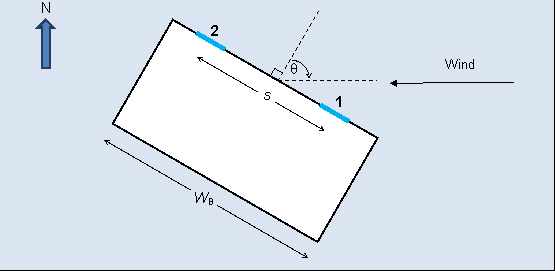
\includegraphics[width=0.9\textwidth, height=0.9\textheight, keepaspectratio=true]{media/ss-figure1.png}
\caption{Plan view of building with 2-opening fa\c{c}ade. \protect \label{fig:ss-plan-view-two-openings}}
\end{figure}

There are two parts to deriving the detailed form of the model:
\begin{enumerate}
\item Express the mean and fluctuating pressures in terms of other physical quantities
that are more readily accessible. EnergyPlus does not have the information on variations
in pressure that is needed to compute $\Delta c_p$ and $\sigma_{\Delta c_p}$. Analysis
of wind tunnel pressure data (Linden et al., 2013) allows for the derivation of simple
expressions for these quantities in terms of the wind direction and opening separation
$s$.\label{ss-item-the-first}
\item Find the coefficients $a_p$ and $a_\sigma$. This is achieved here by analysis of
ventilation rate data (Linden et al., 2013), and using linear regression on the
data.\label{ss-item-the-second}
\end{enumerate}

\subsubsection{Estimation of pressure difference coefficients}
The analysis of pressure data carried out showed that the contributions to the
right-hand side of Equation \ref{eqn:ss-flow-two-terms} can be written to first order
as
\begin{equation}
\Delta c_p=f(s',\theta)
\end{equation}
and
\begin{equation}
\sigma_{\Delta c_p}=g(s',\theta)
\end{equation}
where the dimensionless separation $s' = s/\textup{WB}$,
\begin{equation}
f(s',\theta)=s'\cdot\Pi(\theta),
\end{equation}
and
\begin{equation}
g(s',\theta)=\Sigma_0+s'\cdot\Sigma(\theta).
\end{equation}
That is, to a first approximation the pressure difference mean and standard deviation vary linearly with opening separation, each modulated by its own function of relative wind angle $\theta$.

The formulae for the components are as follows.
\begin{equation}\label{eqn:ss-first-formula}
\Pi(\theta) = 
\begin{cases}
0.44\operatorname{sgn}(\theta)\sin(2.67|\theta|),& |\theta| \leq \theta_0 \\
-0.69 \operatorname{sgn}(\theta)\sin(288-1.6|\theta|),& \theta_0\leq|\theta|\leq\ang{180}.
\end{cases}
\end{equation}
\begin{equation}\label{eqn:ss-second-formula}
\theta_0 = \ang{67.5}
\end{equation}
\begin{equation}\label{eqn:ss-third-formula}
\Sigma(\theta) = 0.423 - 1.63\times 10^{-3}|\theta|
\end{equation}
\begin{equation}\label{eqn:ss-last-formula}
\Sigma_0=0.24
\end{equation}

Figures \ref{fig:ss-figure-2-upper} and \ref{fig:ss-figure-2-lower} show an example of $\Delta c_p$ and $\sigma_{\Delta c_p}$ generated by Equations \ref{eqn:ss-first-formula} through \ref{eqn:ss-last-formula}, respectively, compared with the data.
%
\begin{figure}[hbtp] % fig 2
\centering
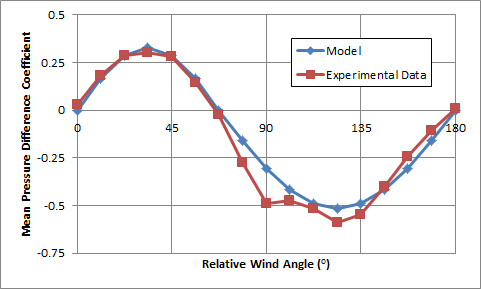
\includegraphics[width=0.9\textwidth, height=0.9\textheight, keepaspectratio=true]{media/ss-chart1.png}
\caption{Mean pressure difference, $\Delta c_p$ predicted by Equations \ref{eqn:ss-first-formula} and \ref{eqn:ss-second-formula}, compared with experimental data. The fa\c{c}ade containing the openings is facing South and the separation is large ($s' = 0.85$). \protect \label{fig:ss-figure-2-upper}}
\end{figure}
%
\begin{figure}[hbtp] % fig 2
\centering
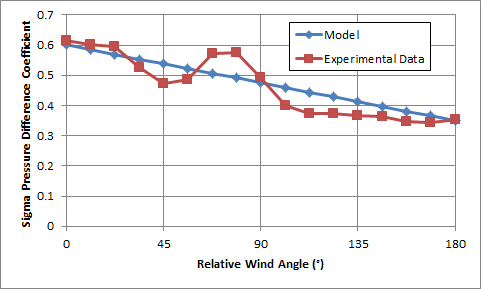
\includegraphics[width=0.9\textwidth, height=0.9\textheight, keepaspectratio=true]{media/ss-chart2.png}
\caption{Standard deviation of pressure difference, $\sigma_{\Delta c_p}$, predicted by Equations \ref{eqn:ss-third-formula} and \ref{eqn:ss-last-formula}, compared with experimental data. The fa\c{c}ade containing the openings is facing South and the separation is large ($s' = 0.85$). \protect \label{fig:ss-figure-2-lower}}
\end{figure}

This completes item \ref{ss-item-the-first} above, i.e. the approximation of the two pressure coefficient terms in Equation \ref{eqn:ss-flow-two-terms} in terms of the dimensionless opening separation and the relative wind angle. There remains item \ref{ss-item-the-second}, i.e. fitting the flow rate data to the formula-generated pressure parameters to determine the constants $a_p$ and $a_\sigma$. When this was carried out, the best fit was found to occur with $a_p = 0.173$ and $a_\sigma = 0.042$. Figure \ref{fig:ss-figure-3-in-original} shows the comparison between the flow rate prediction and the experimental data.

Combining with the previous results we have
\begin{equation}\label{eqn:ss-combined-eqn}
\frac{Q}{A_\text{in} U_\text{ref}}=\left(0.01+\left[0.173 |\Pi(\theta)|+0.042 \Sigma(\theta)\right]s'\right)^{1/2}
\end{equation}

The flow Q is defined to be positive when opening \#1 is the inlet and opening \#2 is the outlet. Since $\Delta p$ is defined as $p_1-p_2$, this can occur when $\Delta c_p > 0$, which in turn corresponds to certain relative wind angles, i.e.
\begin{equation}
\begin{gathered}
Q < 0\ \text{otherwise}\\ 			
Q > 0\ \text{if}\ \ang{0} < \theta < \theta_0\ \text{or}\  \ang{-180} < \theta < -\theta_0
\end{gathered}
\end{equation}

Note that the sense of $Q$ is not necessarily well-defined for all such angles, e.g.
when the unsteady contribution in Equation \ref{eqn:ss-flow-two-terms} is significant:
nevertheless, we retain this definition for all angles.

\begin{figure}[hbtp] % fig 3
\centering
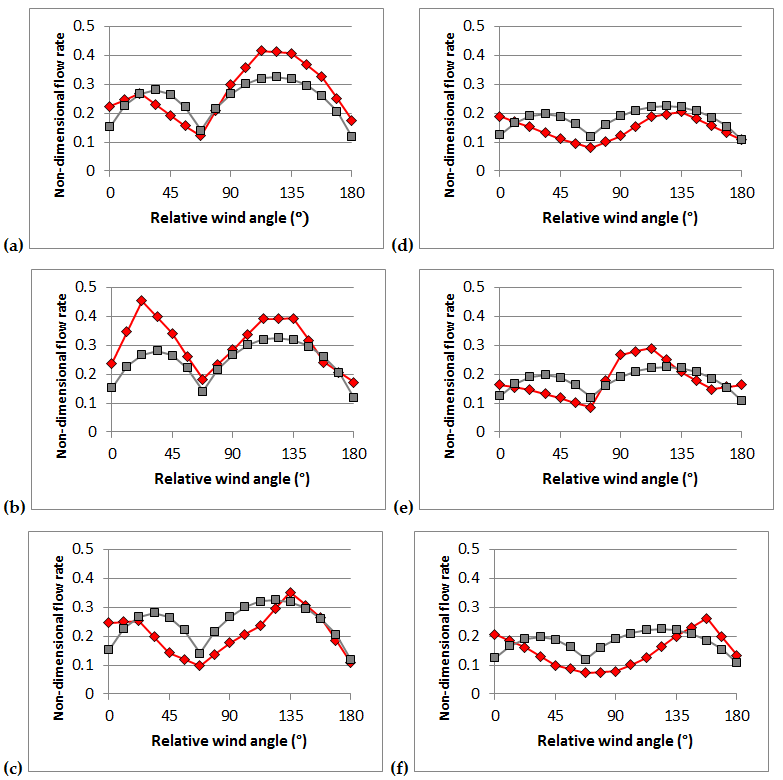
\includegraphics[width=0.9\textwidth, height=0.9\textheight, keepaspectratio=true]{media/ss-figure3.png}
\caption{Comparison of predicted flow rates with experimental data. Each graph shows experimental data (red diamonds) plotted against model prediction (gray squares). Cases in the left-hand column, (a)-(c), are for $s'=0.75$, those in right-hand column, (d)-(f), $s'=0.32$. The three rows are for 2-story isolated, 4-story isolated and 2-story with low density surroundings, respectively. \protect \label{fig:ss-figure-3-in-original}}
\end{figure}

\subsubsection{Inversion of flow rate to equivalent pressure difference}
Finally, we invert the flow rate to obtain the equivalent pressure difference. The purpose of this procedure is to allow incorporation of the model into the network airflow part of EnergyPlus, which requires pressure coefficients to calculate the flow rate: in this way the model will become essentially transparent to the user.
A nodal representation of the 2-aperture single-sided case is shown in Figure \ref{fig:ss-pressure-network-two-openings}.

\begin{figure}[hbtp] % fig 4
\centering
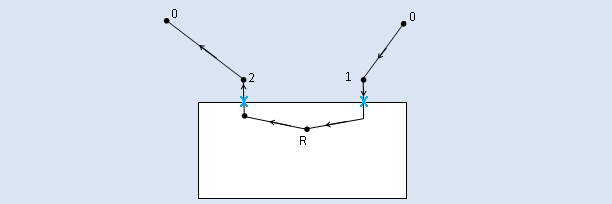
\includegraphics[width=0.9\textwidth, height=0.9\textheight, keepaspectratio=true]{media/ss-figure4.png}
\caption{Pressure network for 2-opening single-sided room. \protect \label{fig:ss-pressure-network-two-openings}}
\end{figure}

Here, 0 is the  ambient, 1 is at the upstream outer surface, 2 is at the downstream outer surface, and R is the room.

Let the openings have areas $A_1$ and $A_2$, not necessarily equal, and a discharge coefficient $C_d$, which is assumed equal, and let $Q$ be the flow rate through the system. Then it can be shown that the pressure difference between the two openings, $\Delta p_{12}$, is related to the flow rate by
\begin{equation}\label{eqn:ss-delta-p-1-2}
\frac{\Delta p_{12}}{\frac{1}{2}\rho V^2} = \frac{1}{C_d^2}\left(\frac{Q/A_\text{eff}}{V}\right)^2
\end{equation}
where the effective area $A_\text{eff}$ is defined by
\begin{equation}
A_\text{eff}=\frac{A_1 A_2}{\left(A_1^2+A_2^2\right)^{1/2}}
\end{equation}
and $V$ is a reference velocity. The left-hand side of Equation \ref{eqn:ss-delta-p-1-2} is a pressure coefficient, $\Delta c_{p,12}^{E+}$, say, and our task is to express this in terms of the flow rate in Equation \ref{eqn:ss-combined-eqn} but using the definition of a pressure coefficient appropriate to EnergyPlus.

The first step is to re-write Equation \ref{eqn:ss-delta-p-1-2} as follows:
\begin{equation}
\Delta c_{p,12}^{E+} = \frac{1}{C_d^2}  \left(\frac{A_\text{in}}{A_\text{eff}}\right)^2 \left(\frac{U_\text{ref}}{V}\right)^2 Q'^2
\end{equation}
where $Q' = Q/(A_\text{in}U_\text{ref})$ is the non-dimensional flow rate of Equation \ref{eqn:ss-combined-eqn}, which is expressed in terms of $Q$, the window area $A_\text{in}$ and the wind speed at 10 m height, $U_\text{ref}$.

The factor $\left(A_\text{in}/A_\text{eff}\right)^2 = 2$, since $A_1 = A_2 = A_\text{in}$, and therefore $A_\text{eff} = A_\text{in}/\sqrt{2}$. The factor $(U_\text{ref}/V)$ relating the velocity scale used in the correlation with that used in the EnergyPlus pressure coefficient may be simplified by noting the following.

EnergyPlus assumes the surface pressure due to wind, $p_w$, is derived from a pressure
coefficient $C_p$ using the local wind speed at \textit{window height}, $V_\text{ref}(z_win)$,
i.e.
\begin{equation}
p_w=\rho_a \left[V_\text{ref}(z_\text{win}\right]^2 C_p/2
\end{equation}
Hence the reference velocity $V =  V_\text{ref}(z_\text{win})$.

EnergyPlus characterizes the vertical wind profile as a power law in z, defined in terms of the local atmospheric boundary layer depth $\delta$ and a power law exponent $\alpha$. EnergyPlus also uses an ``interpolation'' formula to derive the above local wind speed from that measured at the meteorological site, $U_\text{met}$, according to
\begin{equation}
V_\text{ref}(z)= U_\text{met} \left(\frac{\delta_\text{met}}{z}\right)^{\alpha_\text{met}}
\left(\frac{z}{\delta}\right)^\alpha
\end{equation}
where the subscript ``met'' denotes conditions at the meteorological site, and the default values are $z_\text{met} = 10\ \text{m}$, $\delta_\text{met} = 270\ \text{m}$ and $\alpha_\text{met} = 0.14$. The user can change the site parameters from their default values.

The correlation in Equation \ref{eqn:ss-combined-eqn} assumes the reference velocity is the wind speed at 10 m, which will be taken as the local velocity at the building, $V_\text{ref}(10)$.
Combining these results, the pressure coefficient representing the difference in pressure between the two openings is given by
\begin{equation}
\Delta c_{p,12}^{E+} = \frac{1}{C_d^2} \left[ \frac{V_\text{ref}(10)}{V_\text{ref}(z_\text{win})} \right]^2 \left(0.02+\left[0.346 |\Pi(\theta)|+0.084 \Sigma(\theta)\right]{\cdot}s'\right)
\end{equation}
where the velocity ratio
\begin{equation}
\frac{V_\text{ref}(10)}{V_\text{ref}(z_\text{win})} = \left(\frac{10}{z_\text{win}}\right)^\alpha
\end{equation}

Thus, if we assign a pressure coefficient $+0.5\Delta c_{p,12}^{E+}$ to opening 1 and $-0.5\Delta c_{p,12}^{E+}$ to opening 2, then this will provide the necessary pressure difference to give the flow in Equation \ref{eqn:ss-combined-eqn} in a network context.

Note: the pressure coefficient $\Delta c_{p,12}^{E+}$ refers to the difference in pressure between the two openings and is defined in terms of the wind speed at window height. If this is to be combined with a background pressure coefficient for the fa\c{c}ade it is important to ensure the two are defined using the same reference velocity.

\begin{figure}[hbtp] % fig 5
\centering
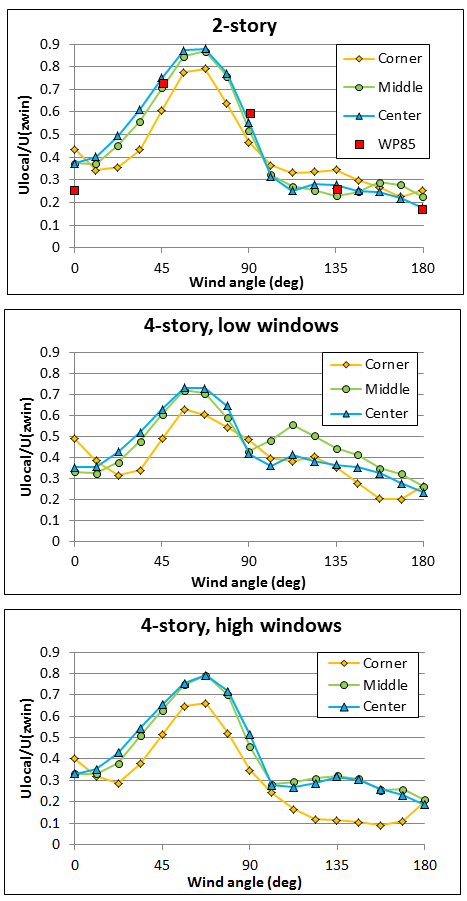
\includegraphics[width=0.9\textwidth, height=0.9\textheight, keepaspectratio=true]{media/ss-figure5.png}
\caption{Local velocity as function of wind angle for wind tunnel data analyzed. On the 2-story graph `WP85' refers to Warren and Parkins (1985), whose measurement location is most closely matched by the ``Center'' curve. \protect \label{fig:ss-local-velocity}}
\end{figure}
%
\begin{figure}[hbtp] % fig 6
\centering
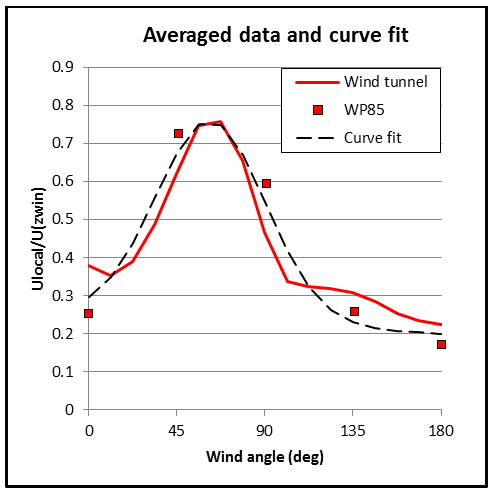
\includegraphics[width=0.9\textwidth, height=0.9\textheight, keepaspectratio=true]{media/ss-figure6.png}
\caption{Wind tunnel data, averaged over all cases, plotted with curve to fit data. \protect \label{fig:ss-wind-tunnel-data}}
\end{figure}

\subsubsection{Testing/Validation/Data Source(s)}
The SS model was developed using wind tunnel pressure and flow rate data acquired by CPP Wind Engineering \& Air Quality Consultants, who carried out two series of tests: (a) Closed Box tests, with a sealed building, to obtain pressure and velocity data and (b) Ventilation tests, with one or two apertures open, to obtain flow rate data. See Linden et al. (2013) for full details.

Each experimental configuration consisted of a cuboidal building with or without a set of blocks representing nearby buildings. 

\begin{itemize}
\item Building: either 2-story, with WB = 47.5 cm, DB = 19.3 cm, HB = 9.9 cm, or 4-story, with HB = 19.8 cm. The model has a nominal scale of 1:70 (based on earlier tests).
\item Environment: building either isolated or at center of a 3 x 3 array of equal-sized blocks, which were of same aspect ratio and either low (2-story height) or high (4-story height), and with either narrow spacing (approximately 0.5WB between blocks) or wide spacing (approximately WB), giving a total of 5 different environments.
\item Approach flow: suburban boundary layer, approximately 10 m/s at 1 m height. The model was mounted on a turntable allowing any desired wind direction to be used. Increments of $\ang{11.25}$ and $\ang{22.5}$ were used for the Closed Box and Ventilation runs, respectively.
\item Room and openings: the building envelope contained a second-floor room of dimensions WRM = 45.9 cm, DRM = 17.7 cm and HRM = 5.0 cm. A total of 15 opening positions were available, distributed around the room. These were sealed for the Closed Box tests but opened in various combinations for the Ventilation runs. 
\item Sensors: 56 pressure transducers, arranged around the opening positions, including 32 at mid-opening height, recorded static pressure, while hot film sensors at 6 different positions recorded flow speed near the surface. For Ventilation runs the decay in concentration of a tracer was measured at two locations inside the room.
\end{itemize}

The data used to develop the model consisted of 6 scenarios: 3 building/environment cases,
\begin{itemize}
\item 2-story isolated building
\item 4-story isolated building
\item 2-story building with low, widely-spaced blocks
\end{itemize}
combined with 2 choices of opening position on the South (long) fa\c{c}ade, namely wide separation ($s' = 0.75$) and medium separation ($s' = 0.32$). 

\subsection{Occupant Ventilation Control}\label{occupant-ventilation-control}

The AirflowNetwork:OccupantVentilationControl object enhances the AirflowNetwork model and provides more practical and advanced controls for window opening and closing operations, based on Marais \& Teichmann (2014). This control includes minimum open and closed time control, indoor thermal comfort control, and opening and closing probability controls.

\subsubsection{Procedures of occupant ventilation control}\label{procedures-of-occupant-ventilation-control}

It should be pointed that the open elapsed time and closed elapsed time are not independent. In other words, when one of the elapsed times value is greater than 0, then other elapsed time value must be equal to 0. The model is either tracking a window as open, in which case the open elapsed time grows, or as closed, in which case the closed elapsed time grows.

The calculation procedures are presented in the following steps:

Step 1: Open elapsed time check

The model checks the open elapsed time first. When the open elapsed time is greater than 0 and less than the minimum opening time, a window will remain open. Otherwise, the model goes to Step 2.

\begin{equation}
Open~elapsed~time~>~minimum~open~time
\end{equation}

Step 2: Closed elapsed time check

This step checks the closed elapsed time. When the closed elapsed time is greater than 0 and less than the minimum closed time, a window will remain closed. Otherwise, the model goes to Step 3.

\begin{equation}
Closed~elapsed~time~>~minimum~closed~time
\end{equation}

Step 3: Elapsed time only?

When either the open elapsed time or the closed elapsed time is long enough (greater than the minimum time) and no other checks are needed, the model returns to the other ventilation control defined in the Ventilation Control Mode field in AirflowNetwork:MultiZone:Zone or AirflowNetwork:MultiZone:Surface. If other checks are needed, the following steps will be performed.

Step 4: Thermal comfort temperature calculation

The thermal comfort check requires the thermal comfort temperature and the comfort band. The comfort temperature of Tcomf is calculated as a function of the outdoor dry-bulb temperature Tout. The comfort temperature calculation may be based on two curves and a boundary temperature point.

\begin{equation}
T_{comf} = \left\{ \begin{array}{ll} \rm{Low Temp Curve,} & \min T_{out} < x \leq \rm{Boundary Point} \\ \rm{High Temp Curve,} & \rm{Boundary Point} \leq x < \max T_{out}  \end{array}\right.
\end{equation}

Step 5: Thermal band calculation

The comfort band is calculated as a function of the design personal dissatisfaction PPD.

\begin{equation}
\theta = -0.0028 \left(100-\rm{PPD}\right)^2 + 0.3419 \left(100-\rm{PPD}\right) - 6.6275
\end{equation}

This equation is valid for PPD 0\% to 35\%

Step 6: Upper boundary check of thermal comfort

After calculation of the comfort temperature and band, the thermal comfort check will be performed using the zone air operative temperature Tg. The check consists of upper and lower boundary checks.

The upper boundary check checks window opening status and uses the following logic:

\begin{equation}
T_g > \left(T_{comf} + \theta\right)
\end{equation}

If the above logic check is true, the opening probability check will be performed. The detailed description is given in the opening probability section.

If the above logic check is false, no action is needed.

If the opening probability check is true and upper boundary check is satisfied, a window will be opened, regardless of open/closed status at the previous time step. If the opening probability check is false and upper boundary check is satisfied, a window will remain at the status from the previous time step.

\begin{equation}
T_g > \left(T_{comf} + \theta\right)~~\&~~\rm{OpeningProbability}
\end{equation}

Step 7: Lower boundary check of thermal comfort

The lower boundary check will follow the upper boundary check to check the window closing status, using the following logic.

\begin{equation}
T_g < \left(T_{comf} - \theta\right)
\end{equation}

If the above logic check is true, the closing probability check will be performed. The detailed description is given in the closing probability section.

If the above logic check is false, no action is needed.

If the closing probability check is true and lower boundary check is satisfied, a window will be closed, regardless of open/closed status at the previous time step. If the closing probability check is false and lower boundary check is satisfied, a window will remain at the status from the previous time step.

\begin{equation}
T_g < \left(T_{comf} - \theta\right)~~\&~~\rm{ClosingProbability}
\end{equation}

The output variables from the model are open status, opening probability status, and closing probability status. The detailed description of opening status is given in the Airflow Network Outputs section in the Input Output Reference.

Note: The upper and lower boundary checks are not independent. In other words, when one of boundary check is satisfied, the other check will be dissatisfied.

\subsubsection{Procedures of opening probability control}\label{procedures-of-opening-probability-control}

Opening probability control provides an optional random number check. The control logic of opening probability is described in the following steps.

Step 1: Closed elapsed time check

This check requires that closed elapsed time is longer than the minimum closing time.

Closed time \textgreater{} minimum closed time

If the time duration is not long enough, the output is false so that a window remains closed.

If the time duration is long enough, an occupancy check is performed.

Step 2: Occupancy check

If a zone is not occupied and the occupancy check is requested, the output is false. If the zone is occupied, the next step is to check the setpoints using zone air temperature at the previous time step as a reference.

Step 3: Setpoint check

There are 5 temperature control types. The following types are available:

\begin{itemize}
\item No control: Bypass
\item Single heating setpoint: If Tzon \textgreater{} setpoint, go to next step. Otherwise, return false.
\item Single cooling setpoint: If Tzon \textless{} setpoint, go to next step. Otherwise, return false.
\item Single heating and cooling setpoint: no action by returning false
\item Dual heating and setpoints: If heating setpoint \textless{} Tzon \textless{} Cooling setpoint, go to next step. Otherwise, return false.
\end{itemize}

Step 4: Select bypass or opening probability check

A choice is provided at this stage so that the opening probability check may be performed or bypassed. If bypassed, the output will be true to open a window. If performed, probability will be determined from a schedule.

Step 5: Perform opening probability check

The opening probability (OP) value is determined from a schedule.

OP = Schedule value or specific function

If the probability value is greater than a random number, the output is true.

OP \textgreater{} random number (random number is between 0 and 1)

Otherwise, the result will be false.

\subsubsection{Procedures of closing probability control}\label{procedures-of-closing-probability-control}

The control logic of closing probability is described as follows.

Step 1: Open elapsed time check

This check requires that open elapsed time is longer than the minimum opening time.

Open time \textgreater{} minimum open time

If the time duration is not long enough, the output is false and the window remains open. Otherwise, Step 2 will be performed.

Step 2: Select by-pass or closing probability check

A choice is provided at this step so that the closing probability check may be performed or bypassed. If bypassed, the output will be true to close a window. If performed, the closing probability will be calculated. The closing probability (CP) value is given from a schedule.

CP = Schedule value or specific function

If the closing probability check is performed and the closing probability is greater than a random number, the output is true.

CP \textgreater{} random number (random number is between 0 and 1)

Otherwise, the result will be false.

\subsection{Pressure Control}\label{pressure-control}

Pressure control is achieved by varying either zone exhaust fan flow rate in a controlled zone or relief air flow rate in an AirLoop. It requires an AirLoop with an OA mixer to reach the pressure setpoint by adjusting a relief air flow, or an OA mixer and an exhaust fan in a controlled zone to reach the pressure setpoint by adjusting an exhaust fan flow rate. The calculation logic is shown below:

1. The AirflowNetwork model will run twice with zero and maximum flow rates for either the controlled zone exhaust fan or relief air flow rate. The controlled zone pressures are the return values.

	In general, the zero flow rate of either exhaust fan or relief node will generate the maximum zone pressure, while the maximum flow rate of either exhaust fan or relief node will produce the minimum zone pressure. 

2. If the setpoint pressure is between the maximum zone pressure caused by zero exhaust fan or relief node flow rate and the minimum zone pressure caused by maximum exhaust fan flow rate or outdoor air flow rate, then the AirflowNetwork model will use root solver to find a solution with calculated zone exhaust fan flow rate or relief node flow rate. Otherwise, the pressure setpoint will not be met. 

3. If both maximum and minimum pressures are higher than the setpoint, the maximum exhaust or outdoor flow rate will be forced. 

4. If both maximum and minimum pressures are lower than the setpoint, then zero flow rate will be forced.

\subsection{References}\label{afn-references}

Atkins, R. E., J. A. Peterka, and J. E. Cermak. 1979. ``Averaged pressure coefficients for rectangular buildings,'' Wind Engineering, Proceedings of the Fifth International Conference 7:369-80, Fort Collins, CO. Pergamon Press, NY.

Awbi, H. B. 2003. Ventilation of Buildings (2\textsuperscript{nd} Edition). Routledge.

Bolmqvist, C. and M. Sandberg, 2004, ``Air Movements through Horizontal Openings in Buildings -- A Model Study,'' International Journal of Ventilation, Vol. 3, No. 1, pp.~1-9.

COMIS Fundamentals. 1990. Edited by Helmut E. Feustel and Alison Rayner-Hooson, LBL-28560, Lawrence Berkeley Laboratory, Berkeley, California.

Conte, S. D. and C de Boor. 1972.Elementary Numerical Analysis: an Algorithmic Approach, McGraw-Hill.

Cooper, L., 1989, ``Calculation of the Flow Through a Horizontal Ceiling/Floor Vent,'' NISTIR 89-4052, National Institute of Standards and Technology, Gaithersburg, Maryland.

Dols, W. S. and G. N. Walton. 2002. ``CONTAMW 2.0 User Manual,'' NISTIR 6921, National Institute of Standards and Technology, Gaithersburg , Maryland.

Holmes, J. D. 1986. Wind Loads on low-rise buildings: The structural and environmental effects of wind on buildings and structures, Chapter 12, Faculty of Engineering, Monash University, Melbourne, Australia.

Linden, P., D. Banks, N. Daish, M. Fountain, G. Gross, A. Honnekeri, M. Pigman, R. Thomas, K. Adams, 
S. Brunswick, S. Dutton, R. Gerard, P. Haves, M. Hovanec, P. Switenki, Y. Zhai, E. Arens, G. Carrilho da Gra\c{c}a, W. Fisk, F. Gillan, M. Hill, T. Lawton, G. Szakats, and H. Zhang. 2016. ``Natural Ventilation for Energy Savings in California Commercial Buildings,'' CEC-500-2016-039, California Energy Commission.

Marais, J. M. and C. Teichmann, ``Window Simulation Methods Required for Manual Window Ventilated Buildings,'' Fifth German-Austrian IBPSA Conference, September 22-24, 2014, RWTH Aachen University, Germany.

Swami, M. V. and S. Chandra. 1988. Correlations for pressure distribution on buildings and calculation of natural-ventilation airflow, ASHRAE Transactions 94(1988) (Pt 1), pp.~243-266.

Swami, M. V., L. Gu, and V. Vasanth. 1992. ``Integration of Radon and Energy Models for Building,'' FSEC-CR-553-92, Florida Solar Energy Center, Cocoa, Florida.

Tan, Q. and Y. Jaluria, 1992, ``Flow through Horizontal Vents as Related to Compartment Fire Environments,'' NIST-GCR-92-607, National Institute of Standards and Technology, Gaithersburg, Maryland.

Walton, G. N. 1989. ``AIRNET -- A Computer Program for Building Airflow Network Modeling,'' NISTIR 89-4072, National Institute of Standards and Technology, Gaithersburg, Maryland.

Walton, G. N. and W. S. Dols. 2003. ``CONTAM 2.1 Supplemental User Guide and Program Documentation,'' NISTIR 7049, National Institute of Standards and Technology, Gaithersburg, Maryland.

Warren, P.R. and Parkins, L.M. (1985) Single-sided ventilation through open windows. In Proceedings of the ASHRAE/DOE/BTECC Conference on Thermal Performance of the Exterior Envelopes of Buildings III, December 2-5, 1985, Clearwater Beach, Florida, pp. 209-228.
